\providecommand{\toplevelprefix}{../..}  %
\documentclass[../../book-main_es.tex]{subfiles}

\begin{document}

\chapter{Métodos de optimización}
\label{app:optimization}

\begin{quote}
    ``{\em Puesto que la estructura del universo es sumamente perfecta y es obra 
        de un Creador sumamente sabio, no ocurre absolutamente nada en el universo 
        en lo que no se manifieste alguna regla de máximo o mínimo.}''

    $~$\hfill -- L. Euler
\end{quote}
\vspace{5mm}

En este capítulo, ofrecemos una breve introducción a algunos de los
algoritmos de optimización más básicos pero importantes que se utilizan en este libro. El
objetivo es únicamente ayudar al lector a aplicar estos algoritmos a los problemas
que se estudian en este libro, no adquirir una comprensión profunda de dichos
algoritmos. Por lo tanto, no proporcionaremos una justificación exhaustiva de
los algoritmos presentados en términos de garantías de rendimiento.

\section{Descenso por gradiente más pronunciado}

La optimización se ocupa de la cuestión de cómo determinar en qué punto una
función, por ejemplo \(\cL(\theta)\), alcanza su valor mínimo.
Matemáticamente, esto se formula como un problema:
\begin{equation}
    \argmin_{\theta \in \Theta} \cL(\theta),
\end{equation}
donde \(\Theta\) representa un dominio al que se limita el argumento \(\theta\).
A menudo (y salvo que se indique lo contrario en este capítulo)
\(\Theta\) es simplemente \(\R^{n}\). Sin pérdida de generalidad,
suponemos que aquí la función \(\cL(\theta)\) es suave\footnote{En
    caso de que la función \(\cL\) no sea suave, reemplazamos su gradiente por
lo que se conoce como \textit{subgradiente}.}.

La eficacia a la hora de encontrar los mínimos (globales) depende de la
información de que dispongamos sobre la función \(\cL\). Para la mayoría de los
problemas de optimización que se tratan en este libro, la dimensión de \(\theta\),
digamos \(n\), es muy grande. Esto hace que calcular o acceder a la información
local sobre \(\cL\) resulte costoso. En particular, dado que el
gradiente \(\nabla \cL\) tiene \(n\) entradas, a menudo resulta razonable
calcularlo; sin embargo, la matriz hessiana \(\nabla^{2} \cL\) tiene \(n^{2}\)
entradas, lo que suele ser totalmente impracticable de calcular (y lo mismo
ocurre con las derivadas de orden superior). Por lo tanto, es habitual suponer
que contamos con la información de orden cero, es decir, que podemos
evaluar \(\cL(\theta)\), y la información de primer orden, es decir, que
podemos evaluar \(\nabla \cL(\theta)\). Los teóricos de la optimización
podrían reformular esto diciendo que tenemos un \textit{«oráculo de primer orden»}. 
Todos los algoritmos de optimización que presentamos en
esta sección solo utilizan un oráculo de primer orden.\footnote{Remitimos a los
    lectores al libro de \cite{Wright-Ma-2022} para una introducción más sistemática
    a los algoritmos de optimización en un espacio de alta dimensión,
incluidos los algoritmos que asumen oráculos de orden superior.}

\subsection{Descenso por gradiente clásico para problemas suaves}

El método más sencillo y más utilizado para la optimización es
el \textit{descenso por gradiente} (GD). Fue introducido por primera vez por Cauchy en
1847. La idea es muy sencilla: partiendo de un estado inicial,
damos pequeños pasos en forma iterativa, de modo que cada paso reduzca el valor de
la función \(\cL(\theta)\).

Supongamos que el estado actual es \(\theta\). Queremos dar un pequeño
paso, digamos de longitud \(h\), en una dirección indicada por un vector
\(\vv\), para llegar a un nuevo estado \(\theta + h\vv\) de tal manera que el valor
de la función disminuya:
\begin{equation}
    \cL(\theta + h\vv) \leq \cL(\theta).
\end{equation}
Para hallar dicha dirección $\vv$, podemos aproximar $\cL(\theta +
h\vv)$ mediante una expansión de Taylor en torno a \(h = 0\):
\begin{equation}
    \cL(\theta + h\vv) = \cL(\theta) + h\ip{\nabla \cL(\theta)}{\vv} + o(h),
\end{equation}
donde el producto interno aquí (y en este capítulo) será el
producto interno \(\ell^{2}\), es decir, \(\ip{\vx}{\vy} = \vx^{\top}\vy\).
Para encontrar la dirección del \textit{gradiente máximo}, intentamos
minimizar esta expansión de Taylor entre los vectores unitarios \(\vv\). Si
\(\nabla \cL(\theta) = \vzero\), entonces el segundo término anterior es \(0\)
independientemente del valor de \(\vv\), por lo que no podemos intentar
avanzar, es decir, el algoritmo ha convergido. Por otro lado, si
\(\nabla \cL(\theta) \neq 0\), entonces se cumple que
\begin{equation}\label{eq:steepest_descent_l2_norm}
    \argmin_{\substack{\vv \in \R^{d} \\ \norm{\vv}_{2} = 1}}
    [\cL(\theta) + h\ip{\nabla \cL(\theta)}{\vv}] =
    \argmin_{\substack{\vv \in \R^{d} \\ \norm{\vv}_{2} = 1}}
    \ip{\nabla \cL(\theta)}{\vv} = -\frac{\nabla
    \cL(\theta)}{\norm{\nabla \cL(\theta)}_{2}},
\end{equation}
En otras palabras, esto significa que el valor de \(\cL(\theta + h\vv)\)
disminuye más rápidamente en la dirección \(\vv = -\nabla \cL(\theta)
/ \norm{\nabla \cL(\theta)}_{2}\), para valores de \(h\) suficientemente pequeños. Esto conduce
al método de descenso por gradiente: a partir del estado actual \(\theta_{k}\)
(\(k=0, 1, \ldots\)), damos un paso de tamaño \(h\) en la dirección
del gradiente negativo para llegar a la siguiente iteración,
\begin{equation}
    \theta_{k+1} = \theta_{k} - h \nabla \cL(\theta_{k}).
\end{equation}
La magnitud del paso \(h\) también se conoce como \textit{tasa de aprendizaje} en
los contextos de aprendizaje automático.

\subsubsection{Selección de la magnitud del paso}

La pregunta que queda por resolver es: ¿cuál debe ser la magnitud del paso \(h\)? Si
elegimos un \(h\) demasiado pequeño, el valor de la función puede disminuir
muy lentamente, como se muestra en el gráfico del centro de
\Cref{fig:step-size}. Si \(h\) es demasiado grande, es posible que el valor ni siquiera
disminuya, como lo muestra el gráfico de la derecha en la \Cref{fig:step-size}.

\begin{figure}[h]
    \centering
    \includegraphics[height=3.5cm]{\toplevelprefix/chapters/appendixA/figs/GD-1.png}
    \hspace{3mm}
    \includegraphics[height=3.5cm]{\toplevelprefix/chapters/appendixA/figs/GD-2.png}
    \hspace{3mm}
    \includegraphics[height=3.5cm]{\toplevelprefix/chapters/appendixA/figs/GD-3.png}
    \caption{El efecto del tamaño de paso (constante) \(h\) en la
    convergencia del método de descenso del gradiente.}
    \label{fig:step-size}
\end{figure}

Por lo tanto, la magnitud del paso \(h\) debe elegirse en función del paisaje de la
función \(\cL(\theta_{k})\). Lo ideal, para elegir el mejor tamaño de paso
\(h\), es resolver el siguiente problema de optimización sobre una sola
variable \(h\):
\begin{equation}
    h = \argmin_{h^{\prime} \geq 0} \cL(\theta_{k} - h^{\prime}\nabla
    \cL(\theta_{k})).
\end{equation}
Este método para elegir el tamaño del paso se denomina \textit{búsqueda lineal};
como sugiere la notación, se suele utilizar para obtener una
tasa de aprendizaje óptima \textit{para cada iteración \(k\)}. Sin embargo, cuando la
función \(\cL(\theta_{k})\) es complicada, lo cual suele ser el
caso al entrenar una red neuronal profunda, esta optimización unidimensional
es muy difícil de resolver en cada iteración del descenso del gradiente.

Entonces, ¿cómo debemos elegir un tamaño de paso adecuado \(h\)? Un enfoque común y
clásico consiste en intentar obtener una buena aproximación del
paisaje local alrededor del estado actual \(\theta\) basándose en cierto
conocimiento sobre el paisaje general de la función \(\cL(\theta)\).

\begin{figure}
    \centering
    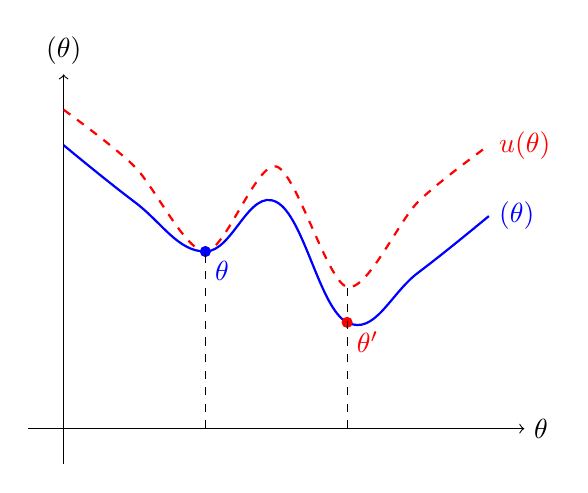
\begin{tikzpicture}[scale=0.9]
        \draw[->] (-0.5,0) -- (6.5,0) node[right] {$\theta$};
        \draw[->] (0,-0.5) -- (0,5) node[above] {$\cL(\theta)$};

        \draw[thick, blue] plot[smooth, tension=0.7] coordinates {
            (0,4) (1,3.2) (2,2.5) (3,3.2) (4,1.5) (5,2.2) (6,3)
        } node[right] {$\cL(\theta)$};

        \draw[thick, red, dashed] plot[smooth, tension=0.5] coordinates {
            (0,4.5) (1,3.7) (2,2.5) (3,3.7) (4,2) (5,3.2) (6,4)
        } node[right] {$u(\theta)$};

        \filldraw[blue] (2,2.5) circle (2pt) node[below right] {$\theta$};

        \filldraw[red] (4,1.5) circle (2pt) node[below right]
        {$\theta^{\prime}$};

        \draw[dashed] (2,0) -- (2,2.5);
        \draw[dashed] (4,0) -- (4,2);
    \end{tikzpicture}
    \caption{\small\textbf{Esquema e intuición de mayorización-minimización.} 
        Una función \(\cL \colon \Theta \to \R\) tiene una
        cota superior global \(u \colon \Theta \to \R\) que se cruza con \(\cL\) en
        al menos un punto \(\theta\). Entonces, encontrar el \(\theta^{\prime}\)
        que minimiza \(u\) mejorará el valor de \(\cL\) a partir de
        \(\cL(\theta)\). Obsérvese que se pueden demostrar resultados similares sobre
    las cotas superiores locales.}
    \label{fig:majorization_minimization}
\end{figure}

Entre las condiciones comunes para el conjunto de definiciones de \(\cL(\theta)\) se cuentan:
\begin{itemize}
    \item Convexidad \(\alpha\)-fuerte. Recordemos que \(\cL\) es
        \textit{\(\alpha\)-fuertemente convexa} si su gráfica se encuentra por encima de una
        cota inferior cuadrática global de pendiente \(\alpha\), es decir,
        \begin{equation}
            \cL(\theta^{\prime}) \geq l_{\theta,
            \alpha}(\theta^{\prime}) \doteq \cL(\theta) + \ip{\nabla
            \cL(\theta)}{\theta^{\prime} - \theta} +
            \frac{\alpha}{2}\norm{\theta^{\prime} - \theta}_{2}^{2}
        \end{equation}
        para cualquier «punto base» \(\theta\). Decimos que \(\cL\) es
        \textit{convexa} si es fuertemente convexa en \(0\), es decir, si su
        gráfico se encuentra por encima de sus tangentes. Es fácil demostrar (la demostración se deja como
        ejercicio) que las funciones fuertemente convexas tienen un único mínimo global.
        Otro hecho importante (demostración como ejercicio) es que
        las funciones dos veces diferenciables y fuertemente convexas en \(\alpha\)
        \(\cL\) tienen Hessianos (simétricos) \(\nabla^{2}\cL\) cuyo
        valor propio mínimo es \(\geq \alpha\). Para \(\alpha > 0\)
        esto implica que la matriz hessiana es simétrica y definida positiva, y
        para \(\alpha = 0\) (es decir, \(\cL\) es convexo) esto implica
        que la matriz hessiana es simétrica y semidefinida positiva.
    \item Gradiente \(\beta\)-Lipschitz (también denominado
        suavidad \(\beta\)). Recordemos que \(\cL\) tiene
        un \textit{\(\beta\)-gradiente Lipschitz} si \(\nabla \cL\)
        existe y es \(\beta\)-Lipschitz, es decir,
        \begin{equation}
            \norm{\nabla \cL(\theta^{\prime}) - \nabla
            \cL(\theta)}_{2} \leq \beta \norm{\theta^{\prime} - \theta}_{2}.
        \end{equation}
        para cualquier «punto base» \(\theta\). Es fácil demostrar (la demostración
        queda como ejercicio) que esto equivale a que \(\cL\) tenga una
        cota superior cuadrática global de pendiente \(\beta\), es decir,
        \begin{equation}
            \cL(\theta^{\prime}) \leq u_{\theta,
            \beta}(\theta^{\prime}) \doteq \cL(\theta) + \ip{\nabla
            \cL(\theta)}{\theta^{\prime} - \theta} +
            \frac{\beta}{2}\norm{\theta^{\prime} - \theta}_{2}^{2}.
        \end{equation}
        para cualquier «punto base» \(\theta\). Otro hecho importante
        (demostración como ejercicio) es que las funciones convexas \(\beta\)-Lipschitz
        con gradiente dos veces diferenciable tienen hessianas (simétricas)
        \(\nabla^{2}\cL\) cuyo mayor valor propio es \(\leq \beta\).
\end{itemize}
En primer lugar, supongamos que \(\cL\) tiene un gradiente \(\beta\)-Lipschitz
(aunque no sea necesariamente convexo). Aprovecharemos esta ocasión para
introducir un tema común en optimización: \textit{para minimizar \(\cL\),
podemos minimizar una cota superior de \(\cL\)}, lo cual se justifica por el
siguiente lema visualizado en la \Cref{fig:majorization_minimization}.
\begin{lemma}[Mayorización-Minimización]\label{lem:majorization_minimization}
    Supongamos que \(u \colon \Theta \to \R\) es una cota superior global
    de \(\cL\), es decir, \(\cL(\theta) \leq u(\theta)\) para todo
    \(\theta \in \Theta\). Supongamos que se igualan en
    \(\theta\), es decir, \(\cL(\theta) = u(\theta)\). Entonces
    \begin{equation}
        \theta^{+} \in \argmin_{\theta^{\prime} \in
        \Theta}u(\theta^{\prime}) \implies \cL(\theta^{+}) \leq
        u(\theta^{+}) \leq u(\theta) = \cL(\theta).
    \end{equation}
\end{lemma}

Utilizaremos este lema para demostrar que podemos recurrir a la propiedad Lipschitz del gradiente 
para garantizar que cada paso del gradiente no empeore el valor de
\(\cL\). De hecho, en cada punto base \(\theta\), tenemos que
\(u_{\theta, \beta}\) es un límite superior global de \(\cL\), y
\(u_{\theta, \beta}(\theta) = \cL(\theta)\). Por lo tanto, por el
\Cref{lem:majorization_minimization}
\begin{equation}
    \text{si \(\theta^{+}\) minimiza \(u_{\theta, \beta}\) entonces}
    \quad \cL(\theta^{+}) \leq u_{\theta, \beta}(\theta^{+}) \leq
    u_{\theta, \beta}(\theta) = \cL(\theta).
\end{equation}
Esto nos lleva a que, al buscar una actualización para obtener \(\theta_{k +
1}\) a partir de \(\theta_{k}\), podamos, en su lugar, minimizar el límite superior
\(u_{\theta_{k}, \beta}\) sobre \(\theta\) y establecer que ese valor sea
\(\theta_{k + 1}\). Al minimizar \(u_{\theta_{k}, \beta}\) (demostración como
ejercicio) obtenemos
\begin{equation}\label{eq:GD}
    \theta_{k + 1} = \theta_{k} - \frac{1}{\beta}\nabla
    \cL(\theta_{k}) \implies \cL(\theta_{k + 1}) \leq \cL(\theta_{k}).
\end{equation}
Esto implica que un tamaño de paso \(h = 1/\beta\) es una tasa de aprendizaje
válida, pero no proporciona una tasa de convergencia ni garantiza que
\(\cL(\theta_{k})\) converja realmente a \(\min_{\theta}\cL(\theta)\).
Esto requiere un poco más de rigor, lo que abordaremos a continuación.

Ahora, supongamos que \(\cL\) es \(\alpha\)-fuertemente convexa, tiene
un gradiente \(\beta\)-Lipschitz y posee un óptimo global
\(\theta^{\star}\). Demostraremos que \(\theta_{k}\) convergerá
directamente al único óptimo global \(\theta^{\star}\), lo cual constituye una
forma muy fuerte de convergencia. En particular, acotaremos
\(\norm{\theta^{\star} - \theta_{k}}_{2}\) utilizando tanto la
convexidad fuerte como la propiedad de Lipschitz del gradiente de \(\cL\), es decir,
analizando el entorno alrededor de \(\theta_{k}\):\footnote{En esta
    demostración, el paso en el que se recurre al gradiente \(\beta\)-Lipschitz es un poco
    complicado. También dejamos este paso como ejercicio, con la pista de
    sustituir \(\theta = \theta_{0} - h\nabla \cL(\theta_{0})\) en la
    identidad del gradiente de Lipschitz.}
\begin{align}
    \norm{\theta^{\star} - \theta_{k + 1}}_{2}^{2}
    &\leq \norm{\theta^{\star} - \theta_{k} + h\nabla
    \cL(\theta_{k})}_{2}^{2} \\
    &= \norm{\theta^{\star} - \theta_{k}}_{2}^{2} + 2h\ip{\nabla
    \cL(\theta_{k})}{\theta^{\star} - \theta_{k}} + h^{2}\norm{\nabla
    \cL(\theta_{k})}_{2}^{2} \\
    &\leq \norm{\theta^{\star} - \theta_{k}}_{2}^{2} +
    2h\bp{\cL(\theta^{\star}) - \cL(\theta_{k}) -
    \frac{\alpha}{2}\norm{\theta^{\star} - \theta_{k}}_{2}^{2}} +
    h^{2}\norm{\nabla \cL(\theta_{k})}_{2}^{2} \quad \text{(\(\alpha\)-SC)} \\
    &= \bp{1 - \alpha h}\norm{\theta^{\star} - \theta_{k}}_{2}^{2} +
    2h(\cL(\theta^{\star}) - \cL(\theta_{k})) + h^{2}\norm{\nabla
    \cL(\theta_{k})}_{2}^{2} \\
    &\leq \bp{1 - \alpha h}\norm{\theta^{\star} - \theta_{k}}_{2}^{2}
    + 2h(\cL(\theta^{\star}) - \cL(\theta_{k})) +
    2h^{2}\beta(\cL(\theta_{k}) - \cL(\theta^{\star})) \quad
    \text{(\(\beta\)-LG)} \\
    &= \bp{1 - \alpha h}\norm{\theta^{\star} - \theta_{k}}_{2}^{2} -
    2h(1 - \beta h)(\cL(\theta_{k}) - \cL(\theta^{\star})).
\end{align}
Para garantizar que la iteración del descenso por gradiente avance,
debemos elegir el tamaño del paso de tal manera que \(1 - \beta h \geq 0\), es decir, \(h
\leq 1/\beta\). Si se da esta condición, entonces
\begin{align}
    \norm{\theta^{\star} - \theta_{k + 1}}_{2}^{2}
    &\leq (1 - \alpha h)\norm{\theta^{\star} - \theta_{k}}_{2}^{2}
    \leq (1 - \alpha h)^{2}\norm{\theta^{\star} - \theta_{k -
    1}}_{2}^{2} \leq \cdots \\
    &\leq (1 - \alpha h)^{k + 1}\norm{\theta^{\star} - \theta_{0}}_{2}^{2}.
\end{align}
Para simplificar el lado derecho, podemos poner \(h = 1/\beta\),
lo que nos da
\begin{equation}
    \norm{\theta^{\star} - \theta_{k + 1}}_{2}^{2} \leq (1 -
    \alpha/\beta)^{k + 1}\norm{\theta^{\star} - \theta_{0}}_{2}^{2},
\end{equation}
que muestra una convergencia exponencial hacia el óptimo global con un error que decrece exponencialmente.
Obsérvese que aquí hemos utilizado una tasa de convergencia para obtener un
\textit{tamaño de paso} adecuado de \(h = 1/\beta\). Este patrón
volverá a aparecer en esta sección.

Terminamos esta sección con una advertencia: encontrar un óptimo global es
(por lo general) una tarea prácticamente imposible. Bajo ciertas condiciones, podemos asegurar
que las iteraciones del descenso por gradiente converjan hacia un \textit{óptimo
local}. Además, bajo condiciones más flexibles, podemos asegurar 
la convergencia \textit{local}, es decir, que las iteraciones converjan a un
óptimo (global o local) si la secuencia se inicializa lo suficientemente cerca
del óptimo.

\subsection{Descenso por gradiente precondicionado para problemas mal condicionados}

\begin{figure}
    \includegraphics[width=\textwidth]{\toplevelprefix/chapters/appendixA/figs/hessian_geometry.png}
    \caption{\small\textbf{El gradiente negativo \(-\nabla
            \cL_{\lambda}\) y el campo vectorial precondicionado (paso del método de Newton)
        \(-[\nabla^{2}\cL_{\lambda}]^{-1}[\nabla \cL_{\lambda}]\)}
        donde \(\lambda = 19\). Hay una zona del espacio en la que
        seguir el campo vectorial del gradiente negativo apenas permite
        avanzar hacia el mínimo, pero en todos los casos, seguir
        el campo vectorial del método de Newton permite avanzar al mismo ritmo
        hacia el óptimo, ya que el gradiente se ha «blanqueado». Dado que
        el hessiano en este caso es diagonal, los algoritmos de tasa de aprendizaje adaptativa
        (por ejemplo, Adam, como se verá más adelante en esta sección) pueden lograr
        un progreso similar al del método de Newton, pero un hessiano no alineado con el eje
    podría incluso impedir que Adam alcance el éxito rápidamente.}
    \label{fig:hessian_geometry}
\end{figure}

\subsubsection{Método de Newton}

Hay algunos problemas suaves y otros fuertemente convexos en los que,
sin embargo, el descenso por gradiente obtiene resultados poco satisfactorios. Por ejemplo, sea
\(\lambda \geq 0\) y sea \(\cL_{\lambda} \colon \R^{2} \to \R\) de la siguiente forma
\begin{equation}
    \cL_{\lambda}(\theta) = \cL_{\lambda}\rp{\mat{\theta_{1}
    \\ \theta_{2}}} \doteq \frac{1}{2}\bc{(1 + \lambda)
    \theta_{1}^{2} + \theta_{2}^{2}} = \frac{1}{2}\theta^{\top}\mat{1
    + \lambda & 0 \\ 0 & 1}\theta.
\end{equation}
Este problema es \(1\)-fuertemente convexo y tiene un gradiente \((1 +
\lambda)\)-Lipschitz. Por lo tanto, la tasa de convergencia es geométrica
con una tasa de \(1 - 1/(1 + \lambda)\). Para valores grandes de \(\lambda\), esto
sigue sin ser muy rápido. En esta sección, presentaremos una clase de
problemas de optimización que pueden optimizar con éxito este tipo de
funciones mal condicionadas.

La clave reside en la \textit{curvatura} del objetivo, que viene dada por
la matriz hessiana. Supongamos (a modo de hipótesis) que tuviéramos un
oráculo de \textit{segundo orden} que nos permitiera calcular
\(\cL(\theta)\), \(\nabla \cL(\theta)\) y
\(\nabla^{2}\cL(\theta)\). Entonces, en lugar de elegir una dirección de descenso
\(\vv\) para optimizar la expansión de Taylor de primer orden alrededor de
\(\theta\), podríamos optimizar la expansión de Taylor de segundo orden
en su lugar. Intuitivamente, esto nos permitiría incorporar información sobre la curvatura
en la actualización.

Hagamos este cálculo. La expansión de Taylor de segundo orden
de \(\cL(\theta + h\vv)\) en torno a \(h = 0\) es
\begin{equation}
    \cL(\theta + h\vv) = \cL(\theta) + h\ip{\nabla \cL(\theta)}{\vv}
    + \frac{1}{2}h^{2}\ip{[\nabla^{2}\cL(\theta)]\vv}{\vv} + o(h^{2}).
\end{equation}
Entonces podemos calcular la dirección de descenso:
\begin{align}
    & \argmin_{\substack{\vv \in \R^{n} \\ \norm{\vv}_{2} =
    1}}\bs{\cL(\theta) + h\ip{\nabla \cL(\theta)}{\vv} +
    \frac{1}{2}h^{2}\ip{[\nabla^{2}\cL(\theta)]\vv}{\vv}} \\
    = &\argmin_{\substack{\vv \in \R^{n} \\ \norm{\vv}_{2} =
    1}}\bs{\ip{\nabla \cL(\theta)}{\vv} +
    \frac{1}{2}h\ip{[\nabla^{2}\cL(\theta)]\vv}{\vv}}.
\end{align}
Este problema de optimización resulta complicado de resolver debido a
la restricción \(\norm{\vv}_{2} = 1\). Pero, en la práctica, nunca
normalizamos la dirección de descenso \(\vv\) y utilizamos el tamaño del paso \(h\)
para controlar la magnitud de la actualización. Así que resolvamos simplemente el problema anterior
para todos los vectores \(\vv \in \R^{n}\):\footnote{Si
    \(\nabla^{2}\cL(\theta)\) no es invertible, entonces podemos sustituir
    \([\nabla^{2}\cL(\theta)]^{-1}\) por la pseudoinversa de Moore-Penrose
de \(\nabla^{2}\cL(\theta)\).}
\begin{equation}
    \argmin_{\vv \in \R^{n}}\bs{\ip{\nabla \cL(\theta)}{\vv} +
    \frac{1}{2}h\ip{[\nabla^{2}\cL(\theta)]\vv}{\vv}} =
    -\frac{1}{h}[\nabla^{2}\cL(\theta)]^{-1}[\nabla \cL(\theta)].
\end{equation}
Por lo tanto, podemos utilizar la iteración del gradiente máximo
\begin{equation}
    \theta_{k + 1} = \theta_{k} -
    [\nabla^{2}\cL(\theta_{k})]^{-1}[\nabla \cL(\theta_{k})],
\end{equation}
(este es el famoso \textit{método de Newton}), o bien
\begin{equation}
    \theta_{k + 1} = \theta_{k} -
    h[\nabla^{2}\cL(\theta_{k})]^{-1}[\nabla \cL(\theta_{k})],
\end{equation}
(conocido como \textit{método de Newton subamortiguado}). Dado que
el término cuadrático de segundo orden \(\cL_{\lambda}\) es igual a su, 
si aplicamos el método de Newton durante \textit{un paso},
alcanzaremos el mínimo global en \textit{un paso} sin importar cuán
grande sea \(\lambda\). La \Cref{fig:hessian_geometry} ofrece una
idea intuitiva sobre las funciones mal condicionadas y los pasos del gradiente
frente a los pasos de Newton.

\subsubsection{PGD}

En la práctica, \textit{no} disponemos de un oráculo de segundo orden que
nos permita calcular \(\nabla^{2}\cL(\theta)\). En su lugar, podemos
intentar \textit{aprender una aproximación de este} junto con la
actualización del parámetro \(\theta_{k + 1}\) a partir de \(\theta_{k}\).

¿Cómo podemos obtener una aproximación a ella? Encontraremos algunas ecuaciones
que la inversa de la matriz hessiana satisfaga y luego intentaremos actualizar nuestra
aproximación para que satisfaga dichas ecuaciones. Concretamente, al tomar la
serie de Taylor de \(\nabla \cL(\theta + \delta_{\theta})\) en torno al
punto \(\theta\), obtenemos
\begin{equation}
    \underbrace{\nabla \cL(\theta + \delta_{\theta}) - \nabla
    \cL(\theta)}_{\doteq \delta_{\vg}} = [\nabla^{2}
    \cL(\theta)]\delta_{\theta} + o(\norm{\delta_{\theta}}_{2}).
\end{equation}
En este caso tenemos
\begin{equation}
    \delta_{\vg} \approx [\nabla^{2}\cL(\theta)]\delta_{\theta}
    \implies \delta_{\theta} \approx [\nabla^{2}\cL(\theta)]^{-1}\delta_{\vg}
\end{equation}
Ahora podemos intentar encontrar una matriz precondicionadora simétrica semidefinida positiva
\(P \in \R^{n \times n}\) tal que
\begin{equation}
    \delta_{\theta} \approx P\delta_{\vg},
\end{equation}
actualizándolo en cada iteración junto con \(\theta_{k}\). Es decir, tenemos
la iteración \textit{PSGD}
\begin{align}
    P_{k}
    &= \mathrm{PreconditionerUpdate}(P_{k - 1}; \theta_{k}, \nabla
    \cL(\theta_{k})) \\
    \theta_{k + 1}
    &= \theta_{k} - hP_{k}\nabla \cL(\theta_{k}).
\end{align}
Esta actualización plantea dos problemas: ¿cómo podemos siquiera utilizar \(P\) (ya que
ya dijimos que no podemos almacenar una matriz \(n \times n\)) y cómo podemos
\textit{actualizar} \(P\) en cada iteración? Las respuestas están muy
relacionadas; nunca podemos materializar \(P\) en la memoria de la computadora, pero
podemos representarla utilizando una factorización de rango bajo (o métodos comparables
    como la \textit{factorización de Kronecker}, que es
particularmente adecuada para la forma de las redes neuronales profundas). A continuación, la
etapa de actualización del precondicionador está diseñada para aprovechar la estructura de
la representación del precondicionador.

Finalizamos esta subsección con una consideración importante: en el aprendizaje profundo, por ejemplo,
\(\cL\) no es una función convexa, por lo que el método de Newton (y
sus aproximaciones) no tienen sentido. En este caso, nos fijamos en la
intuición geométrica del método de Newton en funciones convexas, por ejemplo, a partir de
\Cref{fig:hessian_geometry}: la hessiana inversa \textit{blanquea} los
gradientes. Así, en lugar de un precondicionador que aproxime la hessiana,
podemos ajustar los procedimientos anteriores para aprender una transformación de blanqueo
más general aplicada al gradiente. Esta es la idea en la que se basa la propuesta original
de PSGD \cite{li2017preconditioned}, que contiene más
información sobre cómo almacenar y actualizar el precondicionador, así como
optimizadores más recientes como Muon \cite{liu2025muon}.

\subsection{Descenso por gradiente proximal para problemas no suaves}\label{subsec:pgd}

Sin embargo, incluso en problemas muy sencillos, como el LASSO o el
aprendizaje de diccionarios, el problema no es fuertemente convexo, sino simplemente convexo,
y el objetivo ya no es solo suave, sino más bien la suma de una
función suave y un regularizador no suave (como la
norma \(\ell^{1}\)). Estos problemas se resuelven mediante \textit{algoritmos de optimización proximal}, 
que generalizan el método del gradiente máximo a objetivos no suaves.

En términos formales, digamos que
\begin{equation}
    \cL(\theta) \doteq \cS(\theta) + \cR(\theta)
\end{equation}
donde \(\cS\) es suave, por ejemplo, con un gradiente \(\beta\)-Lipschitz, y
\(\cR\) es no suave (es decir, irregular). El algoritmo del gradiente proximal
generaliza el algoritmo del gradiente máximo, utilizando el
enfoque de mayorización-minimización (es decir,
\Cref{lem:majorization_minimization}) con una cota superior global diferente.
Concretamente, construimos dicho límite superior preguntándonos: ¿qué pasaría si
tomáramos la cota superior del gradiente de Lipschitz de \(S\) pero \textit{dejáramos
\(R\) sin modificar}?  Es decir, tenemos
\begin{equation}
    \cL(\theta^{\prime}) = \cS(\theta^{\prime}) +
    \cR(\theta^{\prime}) \leq u_{\theta, \beta}(\theta^{\prime})
    \doteq \cS(\theta) + \ip{\nabla \cS(\theta)}{\theta^{\prime} -
    \theta} + \frac{\beta}{2}\norm{\theta^{\prime} - \theta}_{2}^{2}
    + \cR(\theta^{\prime}).
\end{equation}
Nótese que (demostración como ejercicio)
\begin{equation}
    \argmin_{\theta^{\prime}}u_{\theta, \beta}(\theta^{\prime}) =
    \argmin_{\theta^{\prime}}\bs{\frac{\beta}{2}\norm*{\theta^{\prime}
        - \bp{\theta - \frac{1}{\beta}\nabla \cS(\theta)}}_{2}^{2} +
    \cR(\theta^{\prime})}.
\end{equation}
Ahora bien, si intentamos minimizar la cota superior \(u_{\theta, \beta}\),
estamos eligiendo un \(\theta^{\prime}\) tal que:
\begin{itemize}
    \item sea similar a la actualización del gradiente \(\theta -
        \frac{1}{\beta}\nabla \cS(\theta)\);
    \item tenga un valor pequeño del regularizador \(\cR(\theta^{\prime})\)
\end{itemize}
y equilibre estas propiedades en función del parámetro de suavidad
\(\beta\). Por consiguiente, definamos el operador proximal
\begin{equation}
    \prox_{h, \cR}(\theta) \doteq
    \argmin_{\theta^{\prime}}\bs{\frac{1}{2h}\norm{\theta^{\prime} -
    \theta}_{2}^{2} + \cR(\theta^{\prime})}.
\end{equation}
A continuación, podemos definir la iteración del \textit{descenso por gradiente proximal}
que, en cada iteración, minimiza el límite superior \(u_{\theta_{k},
h^{-1}}\), es decir,
\begin{equation}
    \theta_{k + 1} = \prox_{h, \cR}(\theta_{k} - h\nabla \cS(\theta_{k})).
\end{equation}
Las demostraciones de convergencia son posibles cuando \(h \leq 1/\beta\), pero
en esta sección no presentamos demostraciones.

Una pregunta que queda por resolver es: ¿cómo podemos calcular el operador proximal? A primera
vista, parece que hemos cambiado un problema de minimización inmanejable por
otro. Dado que hasta ahora no hemos hecho ninguna suposición sobre \(\cR\), el marco
funciona incluso cuando \(\cR\) es una función muy compleja (como una pérdida de red neuronal
), lo que nos obligaría a resolver un problema de entrenamiento de redes neuronales
para calcular un solo operador proximal. Sin embargo, en la práctica, para
regularizadores simples \(\cR\) como los que utilizamos en este artículo, existen
operadores proximales que son fáciles de calcular o que incluso se 
pueden expresar en forma cerrada. A continuación ofrecemos
algunos ejemplos (las demostraciones quedan como ejercicio).

\begin{example}\label{example:prox-of-characteristic-function}
    Sea \(\Gamma \subseteq \Theta\) un conjunto y sea
    \(\chi_{\Gamma}\) la función característica en \(\Gamma\), es decir,
    \begin{equation}
        \chi_{\Gamma}(\theta) \doteq \casework{0, & \text{if}\ \theta
        \in \Gamma \\ +\infty, & \text{if}\ \theta \notin \Gamma.}
    \end{equation}
    Entonces, el operador proximal de \(\chi_{\Gamma}\) es una proyección, es decir,
    \begin{equation}
        \prox_{h, \chi_{\Gamma}}(\theta) = \argmin_{\theta^{\prime}
        \in \Gamma}\frac{1}{2}\norm{\theta^{\prime} - \theta}_{2}^{2}
        = \argmin_{\theta^{\prime} \in \Gamma}\norm{\theta^{\prime} -
        \theta}_{2}.
    \end{equation}
\end{example}

\begin{example}\label{example:prox-of-l1}
    La norma \(\ell^{1}\) tiene un operador proximal que realiza un umbral
    suave:
    \begin{equation}
        S_{h}(\theta) \doteq \prox_{h, \lambda
        \norm{\cdot}_{1}}(\theta) =
        \argmin_{\theta^{\prime}}\bs{\frac{1}{2h}\norm{\theta^{\prime}
        - \theta}_{2}^{2} + \lambda\norm{\theta^{\prime}}_{1}}
    \end{equation}
    entonces \(S_{h}(\theta)\) se define por coordenadas mediante
    \begin{equation}
        S_{h}(\theta)_{i} = \casework{\theta_{i} - h\lambda, &
            \text{if}\ \theta_{i} \geq h\lambda \\ 0, &
            \text{if}\ \theta_{i} \in [-h\lambda, h\lambda] \\ \theta_{i}
        + h\lambda, & \text{if}\ \theta_{i} \leq -h\lambda} =
        \casework{\max\{\abs{\theta_{i}} - h\lambda,
            0\}\sign(\theta_{i}), & \text{if}\ \abs{\theta_{i}} \geq
        h\lambda \\ 0, & \text{if}\ \abs{\theta_{i}} < h\lambda.}
    \end{equation}
    La operación de gradiente proximal en la que la parte suave del
    objetivo es el método de mínimos cuadrados y la parte no suave es la
    norma \(\ell^{1}\) (por lo que se utiliza este operador proximal de umbralización suave)
    se denomina «algoritmo iterativo de contracción y umbralización» (ISTA).
\end{example}

\begin{example}\label{example:prox-of-nonnegative-l1}
    En el \Cref{ch:deep-networks} utilizamos un operador proximal
    correspondiente a la norma \(\ell^{1}\) más la función característica
    del ortante positivo \(\R_{+}^{n} \doteq \{\vx \in
    \R^{n} \colon x_{i} \geq 0\ \forall i\}\), a saber
    \begin{equation}
        T_{h}(\theta) \doteq \prox_{h, \lambda\norm{\cdot}_{1} +
        \chi_{\R_{+}^{n}}}(\theta) = \argmin_{\theta^{\prime} \in
        \R_{+}^{n}}\bs{\frac{1}{2h}\norm{\theta^{\prime} -
        \theta}_{2}^{2} + \lambda\norm{\theta^{\prime}}_{1}},
    \end{equation}
    entonces \(T_{h}\) se define como
    \begin{equation}
        T_{h}(\theta)_{i} \doteq \max\{\theta_{i} - h\lambda, 0\}.
    \end{equation}
    Este operador proximal da como resultado el ISTA no negativo que se
    utiliza en el \Cref{ch:deep-networks} y en otros trabajos posteriores.
\end{example}

\subsection{Descenso de gradiente estocástico para problemas a gran escala}

En el aprendizaje profundo, la función objetivo \(\cL\) no suele poder
calcularse con exactitud, por lo que, en cada paso de optimización, se
\textit{estima} utilizando muestras finitas (por ejemplo, mediante un mini-lote). Una
forma común de modelar esta situación es definir una \textit{función de pérdida estocástica
} \(\cL_{\omega}(\theta)\), donde \(\omega\) es una
``fuente de aleatoriedad''. Por ejemplo, \(\omega\) podría contener los
índices de las muestras de un lote sobre el cual se calcula la pérdida.
Entonces, nos gustaría minimizar \(\cL(\theta) \doteq
\Ex_{\omega}[\cL_{\omega}(\theta)]\) con respecto a \(\theta\), teniendo acceso a
un \textit{oráculo estocástico de primer orden}: dado \(\theta\), podemos
muestrear \(\omega\) y calcular \(\cL_{\omega}(\theta)\) y
\(\nabla_{\theta}\cL_{\omega}(\theta)\). Este problema de minimización se
denomina \textit{problema de optimización estocástica}.

El algoritmo estocástico básico de primer orden es el \textit{descenso estocástico
por gradiente}: en cada iteración \(k\) tomamos una muestra de \(\omega_{k}\),
definimos \(\cL_{k} \doteq \cL_{\omega_{k}}\), y ejecutamos un paso por gradiente
sobre \(\cL_{k}\), es decir,
\begin{equation}
    \theta_{k + 1} = \theta_{k} - h\nabla \cL_{k}(\theta_{k}).
\end{equation}
Sin embargo, incluso para problemas muy sencillos no podemos esperar el mismo tipo
de convergencia que obtuvimos con el descenso por gradiente. Por ejemplo,
supongamos que hay \(m\) valores posibles para \(\omega \in \{1,
\dots, m\}\) que toma con igual probabilidad, y que hay
\(m\) objetivos posibles \(\xi_{1}, \dots, \xi_{m}\), de tal manera que la
función de pérdida \(\cL_{\omega}\) es
\begin{equation}
    \cL_{\omega}(\theta) \doteq \frac{1}{2}\norm{\theta - \xi_{\omega}}_{2}^{2}.
\end{equation}
Entonces, \(\argmin_{\theta}\Ex[\cL_{\omega}(\theta)] = \frac{1}{m}\sum_{i
= 1}^{m}\xi_{i}\), pero el descenso de gradiente estocástico puede «oscilar» alrededor
del valor óptimo global y no converger, tal como se muestra en la
\Cref{fig:sgd_nonconvergence}.

\begin{figure}
    \includegraphics[width=\textwidth]{\toplevelprefix/chapters/appendixA/figs/sgd_vs_nesterov.png}
    \centering
    \caption{\small\textbf{Es posible que el descenso estocástico por gradiente no
            converja, incluso con objetivos muy sencillos, pero el SGD con momentum
        sí converge.} Incluso con objetivos cuadráticos simples, las iteraciones del descenso estocástico
        por gradiente pueden oscilar alrededor del óptimo global,
    mientras que los gradientes promediados por momentum se alinean para apuntar al valor óptimo.}
    \label{fig:sgd_nonconvergence}
\end{figure}

Para solucionar esto, podemos promediar los parámetros
\(\theta_{k}\) o promediar los gradientes \(\nabla
\cL_{k}(\theta_{k})\) a lo largo del tiempo. Si promediamos los parámetros
\(\theta_{k}\), entonces (utilizando \Cref{fig:sgd_nonconvergence} como modelo mental
), el problema del rebote es simplemente imposible,
ya que la iteración promedio tiende a acercarse progresivamente al centro. Por lo tanto,
la mayoría de las demostraciones teóricas de convergencia analizan la convergencia de la
iteración promedio \(\frac{1}{k}\sum_{i = 0}^{k}\theta_{i}\) hacia el
mínimo global. Si promediamos los gradientes, acabaremos obteniendo
un gradiente promedio \(\frac{1}{k}\sum_{i = 0}^{k}\nabla
\cL_{k}(\theta_{k})\), que no cambia mucho en cada iteración
y, por lo tanto, no oscila.

En la práctica, en lugar de utilizar una media aritmética, tomamos una
\textit{media móvil exponencial} (EMA) de los parámetros (esto
se conoce como \textit{promedio de Polyak}) o de los gradientes (esto
se conoce como \textit{«momentum»}). El momentum es más popular y lo estudiaremos aquí.

Una iteración del método de descenso de gradiente estocástico con momentum es la siguiente:
\begin{align}
    \vg_{k}
    &= \beta\vg_{k - 1} + (1 - \beta)\nabla \cL_{k}(\theta_{k}) \\
    \theta_{k + 1}
    &= \theta_{k} - h\vg_{k}.
\end{align}
No vamos a entrar en detalles sobre la demostración de convergencia (véase el capítulo 7 de
\cite{garrigos2023handbook} para ver un ejemplo). Sin embargo, el algoritmo Momentum
resuelve fácilmente nuestro caso de ejemplo de la \Cref{fig:sgd_nonconvergence} (véase la
figura de la derecha): deja de oscilar y, finalmente, converge hacia
el óptimo global.

Terminamos con una advertencia: se puede demostrar que el momentum de Polyak y el momentum de Nesterov
son equivalentes, para ciertas elecciones de los ajustes de los parámetros.
Entonces también es posible demostrar que un esquema de tasa de aprendizaje decreciente
(es decir, la tasa de aprendizaje \(h\) depende de la iteración
\(k\), y su límite es \(h_{k} \to 0\) cuando \(k \to \infty\)) con
SGD simple (o PSGD) puede imitar el efecto del momentum. Es decir,
\cite{defazio2023optimal} demuestra que si el algoritmo SGD dura \(K\)
iteraciones, las normas de los gradientes están acotadas por \(\norm{\nabla
\cL(\theta_{k})}_{2} \leq G\), y definimos \(D \doteq
\norm{\theta_{0} - \theta^{\star}}_{2}\), entonces las iteraciones del SGD simple
\(\theta_{k}\) satisfacen la tasa \(\Ex[\cL(\theta_{k}) -
\cL(\theta^{\star})] \leq DG/\sqrt{K}\) --- pero solo mientras la
tasa de aprendizaje \(h_{k} = (D/[G\sqrt{K}])(1 - k/K)\) decaiga
\textit{linealmente} con el tiempo. Esto concuerda con los esquemas de tasa de aprendizaje
utilizados en la práctica. De hecho, sorprendentemente, dicha teoría de la optimización convexa
puede predecir muchos fenómenos empíricos en las redes profundas
\cite{schaipp2025surprising}, a pesar de que la optimización para aprendizaje profundo
sea altamente no convexa y no suave en el peor de los casos. Hasta el momento
no está claro por qué ocurre esto.

\subsection{Uniéndolo todo: Adam}

El método de descenso por gradiente propone una iteración dada por
\begin{equation}
    \theta_{k + 1} = \theta_{k} + h\vv_{k},
\end{equation}
donde (recordemos) \(\vv_{k}\) se elige para que sea (proporcional al)
vector del gradiente máximo en la norma euclidiana:
\begin{equation}
    \vv_{k} = -\frac{\nabla \cL(\theta_{k})}{\norm{\nabla
    \cL(\theta_{k})}_{2}} \in \argmin_{\substack{\vv \in \R^{n}
    \\ \norm{\vv}_{2} = 1}}\ip{\nabla \cL(\theta_{k})}{\vv}.
\end{equation}
Sin embargo, en el contexto de la optimización del aprendizaje profundo, no hay
absolutamente nada que implique que debamos utilizar la norma euclidiana;
de hecho, la «geometría natural» del espacio de parámetros no se
respeta adecuadamente con la norma euclidiana, ya que pequeños cambios en el
espacio de parámetros pueden dar lugar a diferencias muy grandes en el espacio de salida,
para una entrada fija concreta de la red. Si, en cambio,
utilizáramos una norma genérica \(\norm{\cdot}\) en el espacio de parámetros
\(\R^{n}\), obtendríamos otra cantidad correspondiente a la
denominada \textit{norma dual}:
\begin{equation}
    \vv_{k} \in \argmin_{\substack{\vv \in \R^{n} \\ \norm{\vv} =
    1}}\ip{\nabla \cL(\theta_{k})}{\vv}.
\end{equation}
Por ejemplo, si utilizáramos la norma \(\ell^{\infty}\), es
posible demostrar que
\begin{equation}
    \vv_{k} = -\sign(\nabla \cL(\theta_{k})) \in
    \argmin_{\substack{\vv \in \R^{n} \\ \norm{\vv}_{\infty} =
    1}}\ip{\nabla \cL(\theta_{k})}{\vv},
\end{equation}
donde \(\sign(\vx)_{i} = \sign(x_{i}) \in \{-1, 0, 1\}\). Por lo tanto, si
quisieramos, podríamos utilizar el llamado \textit{descenso por gradiente con signo}:
\begin{equation}\label{eq:sign_gradient_descent}
    \theta_{k + 1} = \theta_{k} - h\sign(\nabla \cL(\theta_{k})).
\end{equation}
A partir del descenso por gradiente de signo, podemos derivar el famoso algoritmo de optimización de Adam.
Obsérvese que, para un escalar \(x \in \R\), podemos escribir
\begin{equation}
    \sign(x) = \frac{x}{\abs{x}} = \frac{x}{\sqrt{x^{2}}}.
\end{equation}
Del mismo modo, para un vector \(\vx \in \R^{n}\) escribimos (donde \(\hada\) y
\(\haddiv\) denotan la multiplicación y la división elemento a elemento)
\begin{equation}
    \sign(\vx) = \vx \haddiv [\vx^{\hada 2}]^{\hada (1/2)}.
\end{equation}
Utilizando esta representación, podemos escribir \eqref{eq:sign_gradient_descent} como
\begin{equation}
    \theta_{k + 1} = \theta_{k} - h ([\nabla \cL(\theta_{k})] \haddiv [\nabla
    \cL(\theta_{k})^{\hada 2}]^{\hada \frac{1}{2}}).
\end{equation}
Ahora consideremos el régimen estocástico en el que optimizamos una
pérdida diferente \(\cL_{k}\) en cada iteración. En el SGD, «seguíamos»
(es decir, tomábamos un promedio de) los gradientes utilizando el momentum. Aquí, podemos
seguir tanto el gradiente como el cuadrado del gradiente utilizando el momentum, es decir,
\begin{align}
    \vg_{k}
    &= \beta^{1}\vg_{k - 1} + (1 - \beta^{1})\nabla \cL_{k}(\theta_{k}) \\
    \vs_{k}
    &= \beta^{2}\vs_{k - 1} + (1 - \beta^{2})[\nabla
    \cL_{k}(\theta_{k})]^{\hada 2}  \\
    \theta_{k + 1}
    &= \theta_{k} - h\vg_{k}\haddiv\vs_{k}^{\hada \frac{1}{2}},
\end{align}
donde \(\beta^{i} \in [0, 1]\) son los parámetros de impulso. El algoritmo
descrito por estas iteraciones es el famoso optimizador 
\textit{Adam},\footnote{Para evitar errores de división por cero, dividimos por
    \(\vs_{k}^{\hada (1/2)} + \eps \vone_{n}\), donde \(\eps\) es pequeño,
digamos del orden de \(10^{-8}\).} que es el optimizador más utilizado en
el aprendizaje profundo. Aunque las demostraciones de convergencia de Adam son más complejas,
se derivan del mismo principio del gradiente máximo que hemos utilizado hasta ahora, por lo que
cabría esperar que, con una tasa de aprendizaje lo suficientemente pequeña, cada
actualización mejorara la pérdida.

Otra forma de entender Adam, que explica en parte su éxito empírico,
es que actualiza dinámicamente las tasas de aprendizaje de cada
parámetro basándose en los gradientes al cuadrado. En particular, fíjate en que
podemos escribir
\begin{equation}
    \theta_{k + 1} = \theta_{k} - \eta_{k} \hada \vg_{k} \qquad \text{where}
    \qquad \eta_{k} = h \vs_{k}^{\hada (-\frac{1}{2})}
\end{equation}
donde \(\eta_{k}\) es la tasa de aprendizaje establecida en forma adaptativa para cada parámetro.
Este esquema se denomina «adaptativo» porque, si el gradiente de un
parámetro concreto es elevado hasta la iteración \(k\), la
tasa de aprendizaje para ese parámetro se reduce para compensar, y
viceversa, como se puede observar en la ecuación anterior.

\section{Cálculo de gradientes mediante diferenciación automática}\label{sec:autodiff}

Anteriormente, analizamos varios algoritmos de optimización para redes profundas
que partían del supuesto de tener acceso a un \textit{oráculo de primer orden}, es decir, un dispositivo
que nos permitiera calcular \(\cL(\theta)\) y \(\nabla
\cL(\theta)\). Para funciones simples de \(\cL\), es posible hacerlo
a mano. Sin embargo, para redes neuronales profundas, esto se vuelve rápidamente
tedioso y dificulta la experimentación rápida. Por lo tanto, necesitamos un
algoritmo general que nos permita calcular de manera eficiente los
gradientes de arquitecturas de redes diferenciables (parcialmente) o "subdiferenciables" arbitrarias.

En esta sección, presentamos los fundamentos de la \textit{diferenciación automática} (AD o \textit{autodiff}), que es un
método computacionalmente eficiente para calcular gradientes y jacobianos de
funciones generales \(f: \R^{m} \to \R^{n}\). Mostraremos cómo esto
conduce al algoritmo de retropropagación para calcular gradientes de
funciones de pérdida que involucran redes neuronales. A continuación se presenta un resumen de la estructura
de esta sección:
\begin{enumerate}
    \item Presentamos los \textbf{diferenciales}, un formalismo práctico
        para calcular y organizar las derivadas de funciones
        entre espacios de parámetros de alta dimensión (que pueden
            ser a su vez productos de otros espacios que involucran matrices,
        tensores, etc.).
    \item Describimos los fundamentos de la diferenciación automática en \textbf{modo directo} y
        \textbf{modo inverso}, lo cual
        implica consideraciones importantes para el cálculo eficiente
        de gradientes y jacobianos para diferentes tipos de
        funciones que surgen en aplicaciones de aprendizaje automático.
    \item Describimos la \textbf{retropropagación} en el caso particular de
        una función de pérdida aplicada a una red neuronal de capas apiladas
        como una instancia de la diferenciación automática en modo reverso.
\end{enumerate}

Nuestro enfoque se inclinará hacia el aspecto matemático, con el fin de proporcionar al lector una
comprensión profunda de los fundamentos matemáticos subyacentes. El lector debe
asegurarse de complementar esta comprensión con un dominio sólido de los aspectos prácticos
de la diferenciación automática para el aprendizaje profundo, tal como se
muestra, por ejemplo, en el excelente tutorial de \textcite{karpathy-micrograd}.

\subsection{Diferenciales}

En la excelente guía
\cite{bright2025matrix} se ofrece una explicación detallada de esta subsección. 
Para introducir el concepto de diferenciales, consideremos primero
el ejemplo sencillo de una función diferenciable \(\cL \colon
\R \to \R\) que depende de un parámetro \(\theta\). Podemos escribir
\begin{equation}
    \cL(\theta^{+}) - \cL(\theta) =
    \cL^{\prime}(\theta)\cdot(\theta^{+} - \theta) +
    o(\abs{\theta^{+} - \theta}).
\end{equation}
Si tomamos \(\delta\theta \doteq \theta^{+} - \theta\) y
\(\delta\cL \doteq \cL(\theta + \delta\theta) - \cL(\theta)\), podemos escribir
\begin{equation}
    \delta\cL = \cL^{\prime}(\theta)\cdot\delta\theta + o(\abs{\delta\theta}).
\end{equation}
Definiremos (de manera no rigurosa) \(\odif{\theta}\) y \(\odif{\cL}\),
es decir, los \textit{diferenciales} de \(\theta\) y \(\cL\), como
cambios \textit{infinitesimalmente pequeños} en \(\theta\) y \(\cL\).
Piensa en ellos como lo que se obtiene cuando \(\delta\theta\) (y, por lo tanto,
\(\delta \cL\)) son extremadamente pequeños. El objetivo del cálculo diferencial,
en cierto sentido, es estudiar las relaciones entre los
diferenciales \(\odif{\theta}\) y \(\odif{\cL}\), es decir, observar
cómo pequeños cambios en la entrada de una función modifican la salida. Debemos
tener en cuenta que el diferencial \(\odif{\theta}\) tiene la
\textit{misma forma} que \(\theta\), y el diferencial
\(\odif{\cL}\) tiene la \textit{misma forma} que \(\cL\). En particular,
podemos escribir
\begin{equation}
    \odif{\cL} = \cL^{\prime}(\theta)\cdot\odif{\theta},
\end{equation}
por lo que se deduce que todas las potencias superiores de \(\abs{\odif{\theta}}\),
como \((\odif{\theta})^{2}\), son \(0\).

Veamos cómo funciona esto en dimensiones superiores, es decir, \(\cL \colon
\R^{n} \to \R\). Entonces seguimos teniendo
\begin{equation}
    \odif{\cL} = \cL^{\prime}(\theta)\cdot\odif{\theta}
\end{equation}
para cierta noción de derivada \(\cL^{\prime}(\theta)\). Dado que
\(\theta\) (y, por lo tanto, \(\odif{\theta}\)) es aquí un vector columna y
\(\cL\) (y, por lo tanto, \(\odif{\cL}\)) es un escalar, se deduce que
\(\cL^{\prime}(\theta)\) es un vector fila. En este caso,
\(\cL^{\prime}(\theta)\) es la jacobiana de \(\cL\)
respecto a \(\theta\). Obsérvese aquí que hemos fijado todas las potencias superiores y
los productos de coordenadas de \(\odif{\theta}\)  en \(0\). En resumen,
\begin{quote}
    \centering
    \textit{Todos los productos y potencias \(\geq 2\) de diferenciales son
    iguales a \(0\).}
\end{quote}

Consideremos ahora una función tensorial de orden superior \(\cL \colon \R^{m \times
n} \to \R^{p \times q}\). Entonces, nuestra ecuación de linealización básica
resulta insuficiente para este caso: \(\odif{\cL} = \cL^{\prime}(\theta) \cdot
\odif{\theta}\) no tiene sentido, ya que \(\theta\) es una matriz de \(m \times
n\), pero \(\odif{\cL}\) es una matriz \(p \times q\), por lo que no hay
ninguna forma de vector o matriz posible para \(\cL^{\prime}(\theta)\) que
funcione en general (ya que ninguna matriz puede multiplicar una matriz \(m \times n\)
para formar una matriz \(p \times q\) a menos que \(m = p\)). Así que debemos tener una
interpretación un poco más avanzada.

Es decir, consideramos \(\cL^{\prime}(\theta)\) como una \textit{transformación lineal}
cuya entrada es el espacio de \(\theta\) y cuya salida es
el espacio de \(\cL\), que toma un pequeño cambio en \(\theta\) y
devuelve el pequeño cambio correspondiente en \(\cL\). Es decir, podemos escribir
\begin{equation}
    \odif{\cL} = \cL^{\prime}(\theta)[\odif{\theta}].
\end{equation}
En los casos anteriores, \(\cL^{\prime}(\theta)\) era primero un operador lineal \(\R \to \R\)
cuya acción consistía en multiplicar su entrada por la
derivada escalar de \(\cL\) con respecto a \(\theta\), y luego un
operador lineal \(\R^{n} \to \R\) cuya acción consistía en multiplicar su
entrada por la derivada jacobiana de \(\cL\) con respecto a
\(\theta\). En general, \(\cL^{\prime}(\theta)\) es la «derivada»
de \(\cL\) con respecto a \(\theta\).
Piensa en \(\cL^{\prime}\) como una versión generalizada de la jacobiana de \(\cL\).
Como tal, sigue algunas reglas de derivación sencillas, entre las que destaca la regla de la cadena.

\begin{theorem}[Regla diferencial de la cadena]
    Supongamos que \(\cL = f \circ g\), donde \(f\) y \(g\) son diferenciables. Entonces
    \begin{equation}
        \odif{\cL} = f^{\prime}(g(\theta))g^{\prime}(\theta)[\odif{\theta}],
    \end{equation}
    donde (como de costumbre) la multiplicación indica la composición de operadores lineales.
    En particular,
    \begin{equation}
        \cL^{\prime}(\theta) = f^{\prime}(g(\theta))g^{\prime}(\theta)
    \end{equation}
    en el sentido de la igualdad de operadores lineales.
\end{theorem}

Resulta útil pensar en la regla de la cadena multivariante en términos functoriales:
la composición de funciones se «convierte» en una multiplicación matricial de jacobianos
(¡la composición de operadores lineales!).
Ilustramos la potencia de este resultado y de esta perspectiva mediante varios
ejemplos.

\begin{example}
    Consideremos la función \(f(\vX) = \vW\vX + \vb\vone^{\top}\). Entonces
    \begin{equation}
        \odif{f} = f(\vX + \odif{\vX}) - f(\vX) = [\vW(\vX +
        \odif{\vX}) + \vb\vone^{\top}] - [\vW \vX + \vb \vone^{\top}]
        = \vW\odif{\vX}.
    \end{equation}
    Por lo tanto, la derivada de una función afín con respecto a su entrada es
    \begin{equation}
        f^{\prime}(\vX)[\odif{\vX}] = \vW\odif{\vX} \implies
        f^{\prime}(\vX) = \vW.
    \end{equation}
    Obsérvese que \(f^{\prime}\) es \textit{constante}. Por otro
    lado, consideremos la función \(g(\vW, \vb) = \vW\vX + \vb\vone^{\top}\). Entonces
    \begin{align}
        \odif{g}
        &= g(\vW + \odif{\vW}, \vb + \odif{\vb}) - g(\vW, \vb)
        \\ 
        &=
        [(\vW + \odif{\vW})\vX + (\vb + \odif{\vb})\vone^{\top}] -
        [\vW\vX + \vb\vone^{\top}] \\
        &= (\odif{\vW})\vX + (\odif{\vb})\vone^{\top} =
        g^{\prime}(\vW, \vb)[\odif{\vW}, \odif{\vb}].
    \end{align}
    Nótese que esta derivada es \textit{constante} en \(\vW, \vb\)
    (lo cual tiene sentido, ya que \(g\) es lineal) y lineal en
    las entradas diferenciales \(\odif{\vW}, \odif{\vb}\).
\end{example}

\begin{example}
    Consideremos la función \(f = gh\), donde \(g\) y \(h\) son
    funciones diferenciables cuyos resultados se pueden multiplicar entre sí.
    Entonces, \(f = p \circ v\), donde \(v = (g, h)\) y \(p(a, b) = ab\).
    Aplicando la regla de la cadena, tenemos
    \begin{equation}
        \odif{f} = p^{\prime}(v(x))v^{\prime}(x)[\odif{x}].
    \end{equation}
    Para calcular \(v^{\prime}(x)\) podemos calcular
    \begin{equation}
        \odif{v} = v^{\prime}(x)[\odif{x}] = v(x + \odif{x}) - v(x) =
        \mat{g(x + \odif{x}) - g(x) \\ h(x + \odif{x}) - h(x)} =
        \mat{g^{\prime}(x)[\odif{x}] \\ h^{\prime}(x)[\odif{x}]}.
    \end{equation}
    Para calcular \(p^{\prime}\), podemos calcular
    \begin{align}
        \odif{p}
        &= p^{\prime}(a, b)[\odif{a}, \odif{b}] = p(a + \odif{a}, b +
        \odif{b}) - p(a, b) = (a + \odif{a})(b + \odif{b}) - ab \\
        &= (\odif{a})b + a(\odif{b}) + (\odif{a})(\odif{b}) =
        (\odif{a})b + a(\odif{b}),
    \end{align}
    donde (recordemos) el producto de las derivadas \(\odif{a}\) y
    \(\odif{b}\) se establece en \(0\). Por lo tanto
    \begin{equation}
        p^{\prime}(a, b)[\odif{a}, \odif{b}] = (\odif{a})b + (\odif{b})a.
    \end{equation}
    Si juntamos todo esto, obtenemos
    \begin{align}
        f^{\prime}(x)[\odif{x}]
        &= p^{\prime}(v(x))v^{\prime}(x)[\odif{x}] = p^{\prime}(g(x),
        h(x))[g^{\prime}(x)[\odif{x}], h^{\prime}(x)[\odif{x}]] \\
        &= (g^{\prime}(x)[\odif{x}])h(x) + g(x)(h^{\prime}(x)[\odif{x}]).
    \end{align}
    Esto da
    \begin{equation}
        f^{\prime}(x)[\odif{x}] = (g^{\prime}(x)[\odif{x}])h(x) +
        g(x)(h^{\prime}(x)[\odif{x}]).
    \end{equation}
    Si, por ejemplo, decimos que \(f, g, h \colon \R \to \R\), entonces
    todo conmuta, por lo que
    \begin{equation}
        f^{\prime}(x)[\odif{x}] = (g^{\prime}(x)h(x) +
        g(x)h^{\prime}(x))[\odif{x}] \implies f^{\prime}(x) =
        g^{\prime}(x)h(x) + g(x)h^{\prime}(x)
    \end{equation}
    que es la conocida regla del producto.
\end{example}

\begin{example}
    Consideremos la función \(f(\vA) = \vA^{\top}\vA\vB\vA\), donde
    \(\vA\) es una matriz y \(\vB\) es una matriz constante. Entonces,
    si ponemos \(f = gh\), donde \(g(\vA) = \vA^{\top}\vA\) y \(h(\vA)
    = \vB\vA\), podemos usar la regla del producto para obtener
    \begin{align}
        f^{\prime}(\vA)[\odif{\vA}]
        &= (g^{\prime}(\vA)[\odif{\vA}])h(\vA) +
        g(\vA)(h^{\prime}(\vA)[\odif{\vA}]) \\
        &= ((\odif{\vA})^{\top}\vA + \vA^{\top}(\odif{\vA}))\vB\vA +
        \vA^{\top}\vA\vB(\odif{\vA}).
    \end{align}
\end{example}

\begin{example}
    Consideremos la función \(f \colon \R^{m \times n \times k} \to
    \R^{m \times n}\) definida por
    \begin{equation}
        f(\vA)_{ij} = \sum_{t = 1}^{k}A_{ijt}.
    \end{equation}
    No podemos escribir una jacobiana (con valores matriciales) ni un gradiente para esta
    función. Pero sí podemos calcular su derivada sin problemas:
    \begin{equation}
        \odif{f}_{ij} = [f(\vA + \odif{\vA}) - f(\vA)]_{ij} = \sum_{t
        = 1}^{k}\odif{\vA}_{ijt} = \vone_{k}^{\top}(\odif{\vA})_{ij}.
    \end{equation}
    Entonces
    \begin{equation}
        (f^{\prime}(\vA)[\odif{\vA}])_{ij} = \vone_{k}^{\top}(\odif{\vA})_{ij},
    \end{equation}
    lo cual representa una operación de multiplicación tensorial de orden superior
    que, no obstante, está bien definida.
\end{example}

Esto nos proporciona toda la tecnología que necesitamos para calcular las derivadas de cualquier cosa.
Lo último que trataremos en esta sección es un método para calcular gradientes utilizando
la derivada. Concretamente, para una función \(\cL\) cuyo resultado es un escalar, el
gradiente \(\nabla \cL\) se define como
\begin{equation}
    \odif{\cL} = \cL^{\prime}(\theta)[\odif{\theta}] = \ip{\nabla
    \cL(\theta)}{\odif{\theta}},
\end{equation}
donde el producto interno aquí es el producto interno «estándar» para
los objetos especificados (es decir, para vectores es el producto interno \(\ell^{2}\),
    mientras que para matrices es el producto interno de Frobenius, y
para tensores de orden superior es el producto interno análogo de suma de coordenadas).
Esta definición es la generalización correcta del ejemplo «familiar» del
gradiente de una función de $\R^n$ a $\R$ como el vector de derivadas parciales:
una versión del teorema de Taylor para funciones generales $f : \R^m \to
\R^n$ hace que esta conexión sea rigurosa.
Así que una forma de calcular el gradiente \(\nabla \cL\) es calcular la diferencial
\(\odif{\cL}\) y reescribirla en la forma
\(\ip{\text{algo}}{\odif{\theta}}\), entonces ese «algo» es el
gradiente.

\subsection{Diferenciación automática}

La idea principal del AD es calcular la regla de la cadena de manera eficiente.
El problema básico al que nos enfrentamos es el siguiente. En la
sección de optimización
del apéndice, consideramos
que el espacio de parámetros \(\Theta\) era un espacio euclidiano abstracto como
\(\R^{n}\). En la práctica, los parámetros son en realidad una colección de vectores,
matrices y objetos de orden superior: \(\Theta = \R^{m \times n} \times \R^{n}
\times \R^{r \times q \times p} \times \R^{r \times q} \times \cdots\). Aunque en
teoría esto equivale a un gran espacio de parámetros \(\R^{n^{\prime}}\) para
algún \(n^{\prime}\) (muy grande), los algoritmos computacionalmente eficientes
para la diferenciación deben tratar estos dos espacios de manera diferente.
La diferenciación automática en modo directo y en modo inverso son dos esquemas distintos para
realizar este cálculo.

Empecemos con un ejemplo sencillo. Sea \(\cL\) definida por \(\cL
= a \circ b \circ c\), donde \(a, b, c\) son diferenciables. Entonces, la
\textit{regla de la cadena} da
\begin{equation}
    \cL^{\prime}(\theta) =
    a^{\prime}(b(c(\theta)))b^{\prime}(c(\theta))c^{\prime}(\theta).
\end{equation}
Para calcular \(\cL(\theta)\), primero calculamos \(c(\theta)\), luego
\(b(c(\theta))\) y después \(a(b(c(\theta)))\), y los guardamos todos. Hay
dos formas de calcular \(\cL^{\prime}(\theta)\). El
\textit{modo directo de AD} calculará
\begin{equation}
    c^{\prime}(\theta) \implies
    b^{\prime}(c(\theta))c^{\prime}(\theta) \implies
    a^{\prime}(b(c(\theta)))b^{\prime}(c(\theta))c^{\prime}(\theta)
\end{equation}
es decir, calculando las derivadas «de abajo hacia arriba». El
\textit{modo inverso de AD} calculará
\begin{equation}
    a^{\prime}(b(c(\theta))) \implies
    a^{\prime}(b(c(\theta)))b^{\prime}(c(\theta)) \implies
    a^{\prime}(b(c(\theta)))b^{\prime}(c(\theta))c^{\prime}(\theta),
\end{equation}
es decir, calcular las derivadas «de arriba hacia abajo». Para ver por qué
esto es importante, supongamos que \(f \colon \R^{p} \to \R^{s}\) viene dada por
\(f = a \circ b \circ c\), donde \(a \colon \R^{r} \to \R^{s}\), \(b
\colon \R^{q} \to \R^{r}\), \(c \colon \R^{p} \to \R^{q}\). Entonces, la
regla de la cadena es:
\begin{equation}
    f^{\prime}(\vx) = a^{\prime}(b(c(\vx)))b^{\prime}(c(\vx))c^{\prime}(\vx)
\end{equation}
donde (recordemos) \(f^{\prime}\) es la derivada, en este caso la
matriz jacobiana (ya que tanto la entrada como la salida de cada función son
vectores). Suponiendo que calcular cada jacobiano es trivial y que el
único costo es multiplicar los jacobianos entre sí, el AD en modo directo tiene
los siguientes costos computacionales (suponiendo que multiplicar \(A \in
\R^{m \times n}, B \in \R^{n \times k}\) toma un tiempo de \(\cO(mnk)\)):
\begin{align}
    &\text{calcular}\ c^{\prime}(\vx) \in \R^{q \times
    p}\ \text{toma un tiempo despreciable} \\
    &\text{calcular}\ b^{\prime}(c(\vx))c^{\prime}(x) \in \R^{r
    \times p}\ \text{toma un tiempo del orden de \(\cO(pqr)\)} \\
    &\text{calcular}\ a^{\prime}(b(c(\vx)))b^{\prime}(c(\vx))c^{\prime}(\vx)
    \in \R^{s \times p}\ \text{toma un tiempo del orden de \(\cO(pqr + prs)\).}
\end{align}
Por otra parte, la diferenciación automática en modo inverso conlleva los siguientes costos computacionales:
\begin{align}
    &\text{calcular}\ a^{\prime}(b(c(\vx))) \in \R^{s \times
    r}\ \text{tima un tiempo despreciable} \\
    &\text{calcular}\ a^{\prime}(b(c(\vx)))b^{\prime}(c(\vx)) \in
    \R^{s \times q}\ \text{toma un tiempo del orden de \(\cO(qrs)\)} \\
    &\text{calcular}\ a^{\prime}(b(c(\vx)))b^{\prime}(c(\vx))c^{\prime}(\vx)
    \in \R^{s \times p}\ \text{toma un tiempo del orden de \(\cO(qrs + pqs)\).}
\end{align}
En otras palabras, el algoritmo de sumas en modo directo tarda un tiempo de orden \(\cO(p(qr + rs))\),
y el algoritmo de sumas en modo inverso tarda un tiempo de orden \(\cO(s(pq + qr))\). \textit{¡Estos
tardan un tiempo diferente!}

En términos más generales, supongamos que \(f = f^{L} \circ \cdots \circ f^{1}\)
donde cada \(f^{\ell} \colon \R^{d^{\ell - 1}} \to \R^{d^{\ell}}\),
de modo que \(f \colon \R^{d^{0}} \to \R^{d^{L}}\). Entonces, el modo directo
tarda \(\cO(d^{0}(\sum_{\ell = 2}^{L}d^{\ell - 1}d^{\ell}))\) tiempo
mientras que el algoritmo de diferenciación automática (AD) en modo reverso tarda \(\cO(d^{L}(\sum_{\ell = 1}^{L -
1}d^{\ell - 1}d^{\ell}))\) tiempo. A partir de las tasas anteriores, vemos que,
en igualdad de condiciones:
\begin{itemize}
    \item Si la función que se va a optimizar tiene \textit{más salidas que
        entradas} (es decir, \(d^{L} > d^{0}\)), utilice \textit{el AD en modo directo}.
    \item Si la función que se va a optimizar tiene \textit{más entradas que
        salidas} (es decir, \(d^{0} > d^{L}\)), utilice \textit{el modo inverso de AD}.
\end{itemize}
En una red neuronal, calculamos el gradiente de una \textit{función de pérdida
} \(\cL \colon \Theta \to \R\), donde el espacio de parámetros
\(\Theta\) suele ser de muy alta dimensión. Por eso, en la práctica siempre
utilizamos la diferenciación automática en modo inverso para entrenar redes 
neuronales. El método de descenso por gradiente en modo inverso, en
el contexto del entrenamiento de redes neuronales, se denomina \textit{retropropagación}.

\subsection{Retropropagación}
\label{app:BP-section}
En esta sección analizaremos la retropropagación algorítmica utilizando un
ejemplo sencillo pero totalmente práctico. Supongamos que fijamos un
par de entrada y etiqueta \((\vX, \vy)\), y fijamos una arquitectura de red
\(f_{\theta} = f_{\theta}^{L} \circ \cdots \circ f_{\theta}^{1} \circ
f_{\theta}^{\emb}\), donde \(\theta = (\theta^{\emb}, \theta^{1},
\dots, \theta^{L}, \theta^{\head})\) y el cabezal específico de la tarea
\(h_{\theta^{\head}}\), y escribimos
\begin{align}
    &\vZ_{\theta}^{1}(\vX) \doteq f_{\theta}^{\emb}(\vX), \\
    &\vZ_{\theta}^{\ell + 1}(\vX) \doteq
    f_{\theta}^{\ell}(\vZ_{\theta}^{\ell}(\vX)), \quad \forall \ell
    \in \{1, \dots, L\}, \\
    &\hat{\vy}_{\theta^{\head}}(\vX) \doteq h_{\theta^{\head}}(\vZ_{\theta}^{L+1}(\vX)).
\end{align}
Entonces, podemos definir la función de pérdida para este ejemplo mediante
\begin{equation}
    \cL(\theta) \doteq \sfL(\vy, \hat{\vy}_{\theta}(\vX)),
\end{equation}
donde \(\sfL\) es una función diferenciable de su segundo argumento.
Entonces, el AD en modo inverso nos indica que calculemos las derivadas en
el orden \(\theta^{\head}, \theta^{L}, \dots, \theta^{1}, \theta^{\emb}\).

Para realizar este cálculo, vamos a introducir algunos cambios en la notación.
\begin{itemize}
    \item En primer lugar, modifiquemos la notación para enfatizar la
        estructura de dependencia entre las variables. Es decir,
        \begin{align}
            &\vZ^{1} \doteq f^{\emb}(\vX, \theta^{\emb}) \\
            &\vZ^{\ell + 1} \doteq f^{\ell}(\vZ^{\ell},
            \theta^{\ell}), \qquad \forall \ell \in \{1, \dots, L\}, \\
            &\hat{\vy} \doteq h(\vZ^{L+1}, \theta^{\head}), \\
            &\cL \doteq \sfL(\vy, \hat{\vy}).
        \end{align}
    \item Entonces, en lugar de escribir la derivada como \(f^{\prime}\),
        denotamos explícitamente la variable independiente y escribimos la
        derivada como \(\odv{f}{\theta^{1}}\), por ejemplo. Esto se debe
        a que hay muchas variables en nuestro modelo y solo 
        nos interesa una a la vez.
\end{itemize}
Podemos empezar calculando las derivadas correspondientes. En primer lugar, para
\(\theta^{\head}\) tenemos
\begin{align}
    \odif{\cL}
    &= \odif{\sfL} \\
    &= \odv{\sfL}{\hat{\vy}}\cdot\odif{\hat{\vy}} \\
    &= \odv{\sfL}{\hat{\vy}}\cdot\odif{{(h(\vZ^{L + 1}, \theta^{\head}))}} \\
    &= \odv{\sfL}{\hat{\vy}}\bs{\odv{h}{\vZ^{L +
        1}}\cdot\odif{\vZ}^{L + 1} +
    \odv{h}{\theta^{\head}}\cdot\odif{\theta}^{\head}}.
\end{align}
Ahora bien, dado que \(\vZ^{L + 1}\) no depende de \(\theta^{\head}\), tenemos
que \(\odif{\vZ}^{L + 1} = 0\), por lo que al final se cumple (utilizando el
    hecho de que el gradiente es la transpuesta de la derivada de una
función \(\sfL\) cuyo codominio es \(\R\)):
\begin{align}
    \odif{\cL}
    &=
    \odv{\sfL}{\hat{\vy}}\cdot\odv{h}{\theta^{\head}}\cdot\odif{\theta}^{\head}
    \\
    &=
    [\nabla_{\hat{\vy}}\sfL]^{\top}\odv{h}{\theta^{\head}}\cdot\odif{\theta}^{\head}
    \\
    &=
    \ip*{\nabla_{\hat{\vy}}\sfL}{\odv{h}{\theta^{\head}}\cdot\odif{\theta}^{\head}}
    \\
    &=
    \ip*{\bp{\odv{h}{\theta^{\head}}}^{*}\nabla_{\hat{\vy}}\sfL}{\odif{\theta}^{\head}}
    \\
    &= \ip{\nabla_{\theta^{\head}}\cL}{\odif{\theta}^{\head}}.
\end{align}
Por lo tanto, para calcular \(\nabla_{\theta^{\head}}\cL\), calculamos el
gradiente \(\nabla_{\hat{\vy}}\sfL\) y el
\textit{adjunto}\footnote{El adjunto es como una transpuesta generalizada
    para transformaciones lineales más generales. En particular, para un
    par dado de espacios con producto interno y una transformación lineal \(T\) entre
    esos espacios, el adjunto \(T^{*}\) se define mediante la identidad
    \(\ip{T\vx}{\vy} = \ip{\vx}{T^{*}\vy}\). En dimensiones finitas (es decir,
todos los casos relevantes para este libro), el adjunto existe y es único.} 
de la derivada \(\odv{h}{\theta^{\head}}\), y los multiplicamos (es decir,
aplicamos la transformación lineal adjunta al gradiente). En
la práctica, ambas derivadas se pueden calcular a mano, pero muchos
marcos computacionales modernos pueden definir \textit{automáticamente} las
derivadas (y/o sus adjuntas) dado el código para la «pasada
directa», es decir, el cálculo de la función de pérdida. Aunque la ampliación de esta
definición automática de la derivada a tantas funciones como sea posible es
un campo de investigación activo, el recurso \cite{bright2025matrix}
describe con cierto detalle un enfoque básico para hacerlo. Por cierto,
la retropropagación también se conoce como el \textit{método adjunto} por esta
razón, es decir, porque utilizamos derivadas adjuntas para calcular el gradiente.

Ahora calculemos las derivadas con respecto a algún \(\theta^{\ell}\):
\begin{align}
    \odif{\cL}
    &= \odv{\cL}{\vZ^{\ell + 1}}\cdot \odif{\vZ^{\ell + 1}} \\
    &= \odv{\cL}{\vZ^{\ell + 1}}\cdot \odif{{(f^{\ell}(\vZ^{\ell},
    \theta^{\ell}))}} \\
    &= \odv{\cL}{\vZ^{\ell +
    1}}\bs{\odv{f^{\ell}}{\vZ^{\ell}}\cdot\odif{\vZ}^{\ell} +
    \odv{f^{\ell}}{\theta^{\ell}}\cdot\odif{\theta}^{\ell}} \\
    &= \odv{\cL}{\vZ^{\ell + 1}}\cdot
    \odv{f^{\ell}}{\theta^{\ell}}\cdot\odif{\theta}^{\ell} \qquad
    \text{(b/c~\(\vZ^{\ell}\) isn't fn.~of \(\theta^{\ell}\) so
    \(\odif{\vZ}^{\ell} = 0\))} \\
    &= [\nabla_{\vZ^{\ell +
    1}}\cL]^{\top}\odv{f^{\ell}}{\theta^{\ell}}\cdot\odif{\theta}^{\ell} \\
    &= \ip*{\nabla_{\vZ^{\ell +
    1}}\cL}{\odv{f^{\ell}}{\theta^{\ell}}\cdot\odif{\theta}^{\ell}} \\
    &= \ip*{\bp{\odv{f^{\ell}}{\theta^{\ell}}}^{*}\nabla_{\vZ^{\ell +
    1}}\cL}{\odif{\theta}^{\ell}} \\
    &= \ip{\nabla_{\theta^{\ell}}\cL}{\odif{\theta}^{\ell}}.
\end{align}
Por lo tanto, para calcular \(\nabla_{\theta^{\ell}}\cL\) calculamos
\(\nabla_{\vZ^{\ell + 1}}\cL\) y luego le aplicamos la derivada adjunta
\(\bp{\odv{f^{\ell}}{\theta^{\ell}}}^{*}\). Dado que
\(\nabla_{\theta^{\ell}}\cL\) depende de \(\nabla_{\vZ^{\ell +
1}}\cL\), también queremos poder calcular los gradientes
con respecto a \(\vZ^{\ell}\). Esto se puede calcular exactamente de la misma manera:
\begin{align}
    \odif{\cL}
    &= \odv{\cL}{\vZ^{\ell + 1}}\cdot \odif{\vZ^{\ell + 1}} \\
    &= \odv{\cL}{\vZ^{\ell + 1}}\cdot\odif{{(f^{\ell}(\vZ^{\ell},
    \theta^{\ell}))}} \\
    &= \odv{\cL}{\vZ^{\ell +
    1}}\bs{\odv{f^{\ell}}{\vZ^{\ell}}\cdot\odif{\vZ}^{\ell} +
    \odv{f^{\ell}}{\theta^{\ell}}\cdot\odif{\theta}^{\ell}} \\
    &= \odv{\cL}{\vZ^{\ell +
    1}}\cdot\odv{f^{\ell}}{\vZ^{\ell}}\cdot\odif{\vZ}^{\ell} \qquad
    \text{(b/c~~\(\theta^{\ell}\) isn't fn.~of \(\vZ^{\ell}\) so
    \(\odif{\theta}^{\ell} = 0\) this time)} \\
    &= \ip*{\bp{\odv{f^{\ell}}{\vZ^{\ell}}}^{*}\nabla_{\vZ^{\ell +
    1}}\cL}{\odif{\vZ}^{\ell}} \qquad \text{(same machine)} \\
    &= \ip{\nabla_{\vZ^{\ell}}\cL}{\odif{\vZ}^{\ell}}.
\end{align}
Por lo tanto, para calcular \(\nabla_{\vZ^{\ell}}\cL\) calculamos
\(\nabla_{\vZ^{\ell + 1}}\cL\) y luego le aplicamos la derivada adjunta
\(\bp{\odv{f^{\ell}}{\vZ^{\ell}}}^{*}\). Así que tenemos una recursión
para calcular \(\nabla_{\vZ^{\ell}}\cL\) para todo \(\ell\), con el caso base
\(\nabla_{\vZ^{L + 1}}\cL\), que viene dado por
\begin{align}
    \odif{\cL}
    &= \odif{\sfL} \\
    &= \odv{\sfL}{\hat{\vy}}\cdot\odif{\hat{\vy}} \\
    &= \odv{\sfL}{\hat{\vy}}\cdot\odif{{h(\vZ^{L + 1}, \theta^{\head})}} \\
    &= \odv{\sfL}{\hat{\vy}}\bs{\odv{h}{\vZ^{L +
        1}}\cdot\odif{\vZ}^{L + 1} +
    \odv{h}{\theta^{\head}}\cdot\odif{\theta}^{\head}} \\
    &= \odv{\sfL}{\hat{\vy}}\cdot \odv{h}{\vZ^{L + 1}}\cdot\odif{\vZ}^{L + 1} \\
    &= \ip*{\bp{\odv{h}{\vZ^{L +
    1}}}^{*}\nabla_{\hat{\vy}}\sfL}{\odif{\vZ}^{L + 1}} \\
    &= \ip{\nabla_{\vZ^{L + 1}}\cL}{\odif{\vZ}^{L + 1}}.
\end{align}
Así, tenemos la recursión:
\begin{align}
    \nabla_{\vZ^{L + 1}}\cL
    &= \bp{\odv{h}{\vZ^{L + 1}}}^{*}\nabla_{\hat{\vy}}\sfL \\
    \nabla_{\vZ^{L}}\cL
    &= \bp{\odv{f^{L}}{\vZ^{L}}}^{*}\nabla_{\vZ^{L + 1}}\cL \\
    \nabla_{\theta^{L}}\cL
    &= \bp{\odv{f^{L}}{\theta^{L}}}^{*}\nabla_{\vZ^{L + 1}}\cL \\
    \vdots &  \\
    \nabla_{\vZ^{1}}\cL
    &= \bp{\odv{f^{1}}{\vZ^{1}}}^{*}\nabla_{\vZ^{2}}\cL \\
    \nabla_{\theta^{1}}\cL
    &= \bp{\odv{f^{1}}{\theta^{1}}}^{*}\nabla_{\vZ^{2}}\cL \\
    \nabla_{\theta^{\emb}}\cL
    &= \bp{\odv{f^{\emb}}{\theta^{\emb}}}^{*}\nabla_{\vZ^{1}}\cL.
\end{align}

Esto nos proporciona un algoritmo computacionalmente eficiente para hallar todos los
gradientes en toda la red.

Terminaremos esta sección calculando la derivada adjunta para una
capa simple.
\begin{example}
    Consideremos la capa «lineal» (afín) \(f^{\ell}\)
    \begin{equation}
        f^{\ell}(\vZ, \vW^{\ell}, \vb^{\ell}) \doteq \vW^{\ell}\vZ +
        \vb^{\ell}\vone^{\top} = \mat{\vW^{\ell} & \vb^{\ell}}.
    \end{equation}
    Podemos calcular las derivadas con respecto a ambos parámetros como
    \begin{align}
        \odif{f}^{\ell}
        &= [(\vW^{\ell} + \odif{\vW}^{\ell})\vZ + (\vb^{\ell} +
        \odif{\vb}^{\ell})\vone^{\top}] - [\vW^{\ell}\vZ + \vb^{\ell}\vone^{\top}] \\
        &= (\odif{\vW}^{\ell})\vZ + (\odif{\vb}^{\ell})\vone^{\top}.
    \end{align}
    Por lo tanto, la derivada de esta transformación es
    \begin{equation}
        \odv{f^{\ell}}{(\vW^{\ell}, \vb^{\ell})}[\odif{\vW}^{\ell},
        \odif{\vb}^{\ell}] = (\odif{\vW}^{\ell})\vZ +
        (\odif{\vb}^{\ell})\vone^{\top},
    \end{equation}
    es decir, que representa la siguiente transformación lineal de
    \(\R^{m \times d} \times \R^{m}\) a \(\R^{m \times n}\):
    \begin{equation}
        T[\vA, \vu] = \vA\vZ + \vu\vone^{\top}.
    \end{equation}
    Calculamos el adjunto \(T^{*} \colon \R^{m \times n} \to \R^{m
    \times d} \times \R^{m}\) con respecto al producto interno
    (de Frobenius) de suma sobre las coordenadas mediante el siguiente procedimiento:
    \begin{align}
        \ip{T[\vA, \vu]}{\vB}_{\R^{m \times n}}
        &= \tr((\vA\vZ + \vu\vone^{\top})\vB^{\top}) \\
        &= \tr(\vA\vZ\vB^{\top} + \vu\vone^{\top}\vB^{\top}) \\
        &= \tr(\vA\vZ\vB^{\top}) + \tr(\vu\vone^{\top}\vB^{\top}) \\
        &= \tr(\vB\vZ^{\top}\vA^{\top}) + \tr(\vone^{\top}\vB^{\top}\vu) \\
        &= \ip{\vB\vZ^{\top}}{\vA}_{\R^{m \times d}} +
        \ip{\vB\vone}{\vu}_{\R^{m}} \\
        &= \ip{\vB(\vZ^{\top}, \vone)}{(\vA, \vu)}_{\R^{m \times d}
        \times \R^{m}}
    \end{align}
    Por lo tanto, \(T^{*}\vB = \vB(\vZ^{\top}, \vone)\).
\end{example}

Es importante destacar que, basándonos en una aplicación simple de la regla de la cadena, tanto la retropropagación
como la diferenciación automática funcionan sobre «grafos computacionales» generales,
es decir, composiciones de funciones (simples). Presentamos todos los
ejemplos como capas de redes neuronales porque este es el ejemplo más común
en la práctica.

\section{Teoría de juegos y optimización minimax}
\label{sec:minimax}\label{sec:game_theory}

En ciertos casos, como en el \Cref{ch:consistent-representations}, un problema de aprendizaje
no puede reducirse a un único problema de optimización, sino que
representa múltiples componentes del sistema, potencialmente opuestos, que intentan
minimizar cada uno su propio objetivo. Entre los ejemplos de este paradigma
se incluyen el aprendizaje de distribuciones mediante redes generativas adversarias
(GAN) y la transcripción en bucle cerrado (CTRL). Denominaremos a dicho
sistema un \textit{juego de dos jugadores}, en el que hay dos «jugadores»
(es decir, componentes) denominados Jugador 1 y Jugador 2 que buscan minimizar
sus propios objetivos \(\cL^{1}\) y \(\cL^{2}\), respectivamente. El Jugador 1
elige los parámetros \(\theta \in \Theta\) y el Jugador 2 elige los parámetros
\(\eta \in \Eta\). En este libro consideramos el caso especial de los
\textit{juegos de suma cero}, es decir, definimos un objetivo común \(\cL\)
tal que \(\cL = -\cL^{1} = \cL^{2}\).

Nuestro primer ejemplo, muy preliminar, es el siguiente. Supongamos que
existen funciones \(u(\theta)\) y \(v(\eta)\) tales que
\begin{equation}
    \cL(\theta, \eta) = -u(\theta) + v(\eta).
\end{equation}
Entonces, los objetivos de ambos jugadores son independientes del otro jugador,
y los jugadores deben intentar alcanzar sus respectivos óptimos:
\begin{equation}
    \theta^{\star} \in \argmin_{\theta \in \Theta}u(\theta), \qquad
    \eta^{\star} \in \argmin_{\eta \in \Eta}v(\eta).
\end{equation}
El par \((\theta^{\star}, \eta^{\star})\) es un caso especial
evidente de un \textit{equilibrio}: una situación en la que ninguno de los
jugadores querrá actuar, si se le presenta la oportunidad, ya que hacerlo acabaría
empeorando su propia situación. Sin embargo, no todos los juegos son tan
triviales; muchos tienen objetivos y estructuras de información más complicados.

En este libro, el formalismo de teoría de juegos pertinente es un juego de Stackelberg
(también denominado juego secuencial). En este formalismo, un
jugador (sin pérdida de generalidad, el Jugador 1, denominado
\textit{líder}) elige sus parámetros antes que el otro (es decir,
Jugador 2, también descrito como un \textit{seguidor}), y el seguidor
puede utilizar todo el conocimiento de la elección del líder para tomar su propia
decisión. La noción correcta de equilibrio para un juego de Stackelberg es un
\textit{equilibrio de Stackelberg}. Para explicar este equilibrio, cabe señalar
que, dado que el Jugador 2 (es decir, el seguidor) puede elegir \(\eta\)
en respuesta a la elección \(\theta_{1}\) realizada por el Jugador 1 (es decir, el
líder), el Jugador 2 elegiría, por supuesto, el \(\eta\) que minimice
\(\cL(\theta_{1}, \cdot)\). Pero, por supuesto, un Jugador 1 racional se
daría cuenta de esto y, por lo tanto, elegiría un \(\theta_{1}\) tal que el peor caso
de \(\eta\) elegido por el Jugador 2 según esta regla no sea tan malo.
De manera más formal, sea \(\cS(\theta) \doteq \argmin_{\eta \in
\Eta}\cL(\theta, \eta)\) el conjunto de valores de \(\eta\) que minimizan
\(\cL(\theta, \eta)\), es decir, el conjunto de todos los valores de \(\eta\) que el Jugador 2
es probable que elija dado que el Jugador 1 ha elegido \(\theta\). Entonces
\((\theta^{\star}, \eta^{\star})\) es un equilibrio de Stackelberg si
\begin{equation}
    \theta^{\star} \in \argmax_{\theta \in \Theta}\min_{\eta \in
    \cS(\theta)}\cL(\theta, \eta), \qquad \eta^{\star} \in
    \argmin_{\eta  \in \Eta}\cL(\theta^{\star}, \eta).
\end{equation}
De hecho (demostración como ejercicio), se puede demostrar que, en el contexto de
los juegos de Stackelberg de suma cero para dos jugadores, \((\theta^{\star},
\eta^{\star})\) es un equilibrio de Stackelberg si y solo si
\begin{equation}
    \theta^{\star} \in \argmax_{\theta \in \Theta}\min_{\eta \in
    \Eta}\cL(\theta, \eta), \qquad \eta^{\star} \in \argmin_{\eta
    \in \Eta}\cL(\theta^{\star}, \eta),
\end{equation}
(nótese que la notación \(\cS(\theta)\) no se utiliza ni es necesaria).
\begin{proof} %
    Nótese que 
    \begin{equation}
        \cS(\theta) = \argmin_{\eta \in \Eta}\cL(\theta, \eta),
    \end{equation}
    por lo que se cumple que
    \begin{equation}
        \min_{\eta \in \cS(\theta)}\cL(\theta, \eta) = \min_{\eta \in
            \argmin_{\eta^{\prime} \in \Eta}\cL(\theta,
        \eta^{\prime})}\cL(\theta, \eta) = \min_{\eta \in
        \Eta}\cL(\theta, \eta).
    \end{equation}
\end{proof}

En el resto de esta sección, analizaremos brevemente algunos enfoques algorítmicos
para aprender puntos de equilibrio de Stackelberg. La intuición central
es que aprender un equilibrio es como dejar que las diferentes
partes del sistema determinen automáticamente las compensaciones entre los
diferentes objetivos que desean optimizar.

Terminamos esta sección con una advertencia: en los juegos de suma cero para dos jugadores, si
se cumple que
\begin{equation}
    \max_{\theta \in \Theta}\min_{\eta \in \Eta}\cL(\theta, \eta) =
    \min_{\eta \in \Eta}\max_{\theta \in \Theta}\cL(\theta, \eta)
\end{equation}
entonces todo equilibrio de Stackelberg es un punto de 
silla,\footnote{Conocido como \textit{equilibrio de Nash}.} es decir,
\begin{equation}
    \theta^{\star} \in \argmax_{\theta \in \Theta}\cL(\theta,
    \eta^{\star}), \qquad \eta^{\star} \in \argmin_{\eta \in
    \Eta}\cL(\theta^{\star}, \eta),
\end{equation}
\textit{y viceversa}, y además cada equilibrio de Stackelberg
tiene el (mismo) valor objetivo \[\max_{\theta \in \Theta}\min_{\eta
\in \Eta}\cL(\theta, \eta).\]
\begin{proof} %
    Supongamos que, efectivamente,
    \begin{equation}
        \max_{\theta \in \Theta}\min_{\eta \in \Eta}\cL(\theta, \eta)
        = \min_{\eta \in \Eta}\max_{\theta  \in \Theta}\cL(\theta, \eta).
    \end{equation}

    Supongamos primero que \((\theta^{\star}, \eta^{\star})\) es un punto de silla.
    Demostraremos que se trata de un equilibrio de Stackelberg. Por definición, tenemos
    \begin{equation}
        \min_{\eta \in \Eta}\cL(\theta^{\star}, \eta) =
        \cL(\theta^{\star}, \eta^{\star}) = \max_{\theta \in
        \Theta}\cL(\theta, \eta^{\star}).
    \end{equation}
    Por lo tanto, se cumple para cualquier \(\theta\) y \(\eta\) que
    \begin{equation}
        \min_{\eta \in \Eta}\cL(\theta, \eta) \leq \cL(\theta,
        \eta^{\star}) \leq \cL(\theta^{\star}, \eta^{\star}).
    \end{equation}
    Por lo tanto
    \begin{equation}
        \max_{\theta \in \Theta}\min_{\eta \in \Eta}\cL(\theta, \eta) \leq
        \cL(\theta^{\star}, \eta^{\star}).
    \end{equation}
    De manera totalmente simétrica,
    \begin{equation}
        \cL(\theta^{\star}, \eta^{\star}) \leq \cL(\theta^{\star},
        \eta) \leq \max_{\theta \in \Theta}\cL(\theta, \eta)
        \implies \cL(\theta^{\star}, \eta^{\star}) \leq \min_{\eta
        \in \Eta}\max_{\theta \in \Theta}\cL(\theta, \eta).
    \end{equation}
    Por lo tanto, dado que \(\max\min = \min\max\), tenemos
    \begin{equation}\label{eq:nash_equilibrium_minmax_maxmin}
        \max_{\theta \in \Theta}\min_{\eta \in \Eta}\cL(\theta, \eta)
        = \cL(\theta^{\star}, \eta^{\star}) = \min_{\eta \in
        \Eta}\max_{\theta \in \Theta}\cL(\theta, \eta).
    \end{equation}
    En particular, se cumple que
    \begin{equation}
        \theta^{\star} \in \argmax_{\theta \in \Theta}\min_{\eta \in
        \Eta}\cL(\theta, \eta).
    \end{equation}
    A partir de la condición del punto de silla, tenemos que \(\eta^{\star} \in
    \argmin_{\eta \in \Eta}\cL(\theta^{\star}, \eta)\). Por lo tanto,
    \((\theta^{\star}, \eta^{\star})\) es un equilibrio de Stackelberg.
    Además, también hemos demostrado que todos los puntos de silla obedecen a
    \eqref{eq:nash_equilibrium_minmax_maxmin}.

    Supongamos ahora que \((\theta^{\star}, \eta^{\star})\) es un equilibrio de Stackelberg.
    Afirmamos que se trata de un punto de silla, lo que completa
    la demostración. Por la definición de equilibrio minimax,
    \begin{equation}
        \max_{\theta \in \Theta}\min_{\eta \in \Eta}\cL(\theta, \eta)
        = \cL(\theta^{\star}, \eta^{\star}).
    \end{equation}
    Entonces, por la suposición de que \(\min\max = \max\min\), tenemos
    \begin{equation}
        \max_{\theta \in \Theta}\min_{\eta \in \Eta}\cL(\theta, \eta)
        = \cL(\theta^{\star}, \eta^{\star}) = \min_{\eta \in
        \Eta}\max_{\theta \in \Theta}\cL(\theta, \eta).
    \end{equation}
    Esto demuestra que todos los equilibrios minimax tienen el valor objetivo deseado
    \(\cL(\theta^{\star}, \eta^{\star})\). Ahora queremos
    demostrar que
    \begin{equation}
        \theta^{\star} \in \argmax_{\theta \in \Theta}\cL(\theta,
        \eta^{\star}), \qquad \eta^{\star} \in \argmin_{\eta \in
        \Eta}\cL(\theta^{\star}, \eta).
    \end{equation}
    De hecho, esta última afirmación se cumple por definición del equilibrio minimax,
    por lo que solo es necesario demostrar la primera. Es decir, demostraremos que
    \begin{equation}
        \max_{\theta \in \Theta}\cL(\theta, \eta^{\star}) =
        \cL(\theta^{\star}, \eta^{\star}).
    \end{equation}
    Para demostrar esto, basta con que, por definición de \(\max\)
    \begin{equation}
        \cL(\theta^{\star}, \eta^{\star}) \leq \max_{\theta \in
        \Theta}\cL(\theta, \eta^{\star}),
    \end{equation}
    Por otra parte, tenemos que \(\min_{\eta \in \Eta}\cL(\theta, \eta) \leq
    \cL(\theta, \eta^{\star})\), por lo que
    \begin{equation}
        \cL(\theta^{\star}, \eta^{\star}) = \max_{\theta \in
        \Theta}\min_{\eta \in \Eta}\cL(\theta, \eta) \leq
        \max_{\theta \in \Theta}\cL(\theta, \eta^{\star}).
    \end{equation}
    Por lo tanto, se cumple que
    \begin{equation}
        \cL(\theta^{\star}, \eta^{\star}) = \max_{\theta \in
        \Theta}\cL(\theta, \eta^{\star}),
    \end{equation}
    y con esto queda completada la demostración.
\end{proof}
Las condiciones bajo las cuales se cumple la igualdad \(\min\max = \max\min\)
vienen dadas por los llamados \textit{teoremas del minimax}; el más destacado
de ellos es un teorema de von Neumann. Sin embargo, en los casos que nos
ocupan, esta propiedad no suele cumplirse.

\subsection{El aprendizaje de los equilibrios de Stackelberg}

¿Cómo podemos aprender puntos de equilibrio de Stackelberg mediante GDA? En general, esto es
claramente imposible, ya que aprender equilibrios de Stackelberg mediante GDA es
obviamente al menos tan difícil como calcular un minimizador global de una función de pérdida
(por ejemplo, estableciendo que el objetivo compartido \(\cL(\theta, \eta)\)
sea únicamente una función de \(\eta\)). Por lo tanto, podemos lograr dos tipos
de garantías de convergencia:
\begin{itemize}
    \item Cuando \(\cL\) es (fuertemente) cóncava respecto al primer argumento
        \(\theta\) y (fuertemente) convexa respecto al segundo argumento
        \(\eta\) (además de tener gradientes de Lipschitz con respecto a ambos
        argumentos), podemos lograr una convergencia exponencial hacia
        un equilibrio de Stackelberg.
    \item Cuando \(\cL\) no es cóncava ni convexa en ninguno de los argumentos,
        podemos obtener \textit{garantías de convergencia local}: es decir,
        si inicializamos los valores de los parámetros cerca de un equilibrio
        de Stackelberg (local) y la geometría de optimización es adecuada,
        entonces podemos aprender ese equilibrio de manera eficiente.
\end{itemize}

La primera situación es exactamente análoga al caso de
la optimización de un solo jugador, donde demostramos que el descenso por gradiente
converge exponencialmente para objetivos fuertemente convexos que
tienen un gradiente Lipschitz. La segunda situación también es análoga al
caso de la optimización de un solo jugador, aunque no la tratamos
en profundidad debido a la dificultad técnica; de hecho, existen garantías de
convergencia local para objetivos no convexos que tienen una geometría
localmente favorable.

El algoritmo en estos dos casos es el mismo, denominado
descenso-ascenso por gradiente (GDA). Para entender el GDA, supongamos que estamos tratando
de aprender \(\theta^{\star}\). Podríamos aplicar el ascenso por gradiente a la
función \(\theta \mapsto \min_{\eta \in \Eta}\cL(\theta, \eta)\).
Pero entonces tendríamos que tomar la derivada con respecto a \(\theta\) de esta
función. Para ver cómo hacerlo, supongamos que \(\cL\) es fuertemente
convexa en \(\eta\), de modo que existe un minimizador
\(\eta^{\star}(\theta)\) de \(\cL(\theta, \cdot)\). Entonces,
\textit{el teorema de Danskin} establece que
\begin{equation}
    \nabla_{\theta}\bs{\min_{\eta \in \Eta}\cL(\theta, \eta)} =
    \nabla_{\theta}\cL(\theta, \texttt{stop\_grad}(\eta^{\star}(\theta))),
\end{equation}
donde el gradiente es \textit{solo con respecto al primer
argumento} (es decir, no es una derivada total, lo que requeriría calcular
la jacobiana de \(\eta^{\star}(\theta)\) con respecto a \(\theta\)),
lo que se indica mediante el operador stop-gradient.\footnote{En el caso de que
    \(\cL\) no sea fuertemente convexa en \(\eta\), sino simplemente convexa,
    el teorema de Danskin puede expresarse en términos de subdiferenciales. Si
    \(\cL\) no es convexa en absoluto en \(\eta\), entonces esta derivada puede
    no estar bien definida, pero de todos modos se pueden obtener garantías de convergencia
    (local) para el algoritmo resultante. Por lo tanto, utilizamos
    el teorema de Danskin como motivación y no como justificación para nuestros
    algoritmos. Los teoremas de Danskin pueden generalizarse a situaciones más flexibles
mediante los denominados \textit{teoremas de envoltura}.}
Para derivar con respecto a \(\theta\), necesitamos establecer un
\textit{proceso secundario} que también optimice \(\eta\) a fin de obtener una
aproximación de \(\eta^{\star}(\theta)\). Podemos hacerlo mediante
la siguiente plantilla algorítmica:
\begin{align}
    &\eta_{k + 1} = \eta_{k + 1}^{T + 1}; \qquad \eta_{k + 1}^{t + 1}
    = \eta_{k + 1}^{t} - h \nabla_{\eta} \cL(\theta_{k}, \eta_{k +
    1}^{t}), \quad \forall t \in [T]; \qquad \eta_{k + 1}^{1} = \eta_{k} \\
    &\theta_{k + 1} = \theta_{k} + h \nabla_{\theta}\cL(\theta_{k},
    \eta_{k + 1}).
\end{align}
Es decir, damos \(T\) pasos de descenso por gradiente para actualizar
\(\eta_{k}\) (con la esperanza de llegar al mínimo de \(\cL(\theta_{k},
\cdot)\)), y luego damos un paso de ascenso por gradiente para actualizar
\(\theta_{k}\). Como ventaja adicional, además de estimar \(\theta_{K} \approx
\argmax_{\theta}\min_{\eta}\cL(\theta, \eta)\), también aprendemos un
\(\eta_{K} \approx \argmin_{\eta}\cL(\theta_{K}, \eta)\) --- esto es
un equilibrio de Stackelberg aproximado.

En la práctica, este método no suele utilizarse, ya que requiere \(T + 1\)
iteraciones totales de descenso por gradiente para actualizar \(\theta\) una sola vez. En su lugar,
utilizamos la denominada iteración de \textit{descenso-ascenso por gradiente (simultáneo)}
(GDA)
\begin{align}
    \theta_{k + 1}
    &= \theta_{k} + h\nabla_{\theta}\cL(\theta_{k}, \eta_{k}) \\
    \eta_{k + 1}
    &= \eta_{k} - Th\nabla_{\eta}\cL(\theta_{k}, \eta_{k}),
\end{align}
lo cual se puede implementar de manera eficiente mediante un único paso de gradiente en
\((\theta, \eta)\). La idea clave aquí es que, para que nuestro método
se acerque a la iteración ineficiente anterior, utilizamos una actualización de \(\eta\)
que es \(T\) veces más rápida que la actualización de \(\theta\) (estas pueden
considerarse prácticamente iguales si se linealiza la dinámica).

Es fundamental elegir \(T\) de manera sensata. ¿Cómo podemos hacerlo? A continuación,
analizamos dos configuraciones de \(T\) que conducen a
la convergencia del GDA hacia un equilibrio de Stackelberg bajo diferentes supuestos.

\subsubsection{Convergencia del GDA de escala única de tiempo hacia el equilibrio de Stackelberg}

Si \(T = 1\) (es decir, denominado \textit{de escala de tiempo única} porque tanto
las actualizaciones de \(\theta\) como las de \(\eta\) son de la misma escala), entonces el algoritmo GDA
se convierte en
\begin{equation}
    \theta_{k + 1} = \theta_{k} + h\nabla_{\theta}\cL(\theta_{k},
    \eta_{k}), \qquad \eta_{k + 1} = \eta_{k} -
    h\nabla_{\eta}\cL(\theta_{k}, \eta_{k}).
\end{equation}
Si \(\cL\) tiene gradientes de Lipschitz en \(\theta\) y \(\eta\), y es
fuertemente cóncava en \(\theta\) y fuertemente convexa en \(\eta\), y
es coercitiva (es decir, \(\lim_{\norm{\theta}_{2}, \norm{\eta}_{2} \to
\infty}\cL(\theta, \eta) = \infty\)), entonces todos los puntos de silla son
equilibrios de Stackelberg y viceversa. El trabajo
\cite{zamani2024convergence} demuestra que el GDA (de nuevo, con \(T = 1\))
con un tamaño de paso \(h\) suficientemente pequeño converge a un punto de silla
(y, por lo tanto, a un equilibrio de Stackelberg) a una velocidad exponencial si existe alguno,
en forma análoga al descenso por gradiente para funciones fuertemente convexas con
gradiente de Lipschitz.\footnote{No proporcionamos el tamaño del paso ni
    la base exponencial, ya que se trata de funciones complejas de la
    constante de convexidad/concavidad/Lipschitz del gradiente. Por supuesto,
    el artículo \cite{zamani2024convergence} ofrece los valores exactos de los parámetros.} 
Según nuestro conocimiento, este tipo de resultados constituye la única
justificación rigurosa conocida para el GDA de escala temporal única.

\subsubsection{Convergencia local del GDA de doble escala de tiempo hacia el
equilibrio de Stackelberg}

La convexidad/concavidad fuerte es una propiedad \textit{global}, y ninguno de
los juegos que analizamos en este libro tiene objetivos que sean
globalmente fuertemente cóncavos/fuertemente convexos. En este caso, lo mejor que
podemos esperar es una convergencia \textit{local} hacia equilibrios de Stackelberg:
si los parámetros se inicializan cerca de un equilibrio de Stackelberg,
entonces el GDA puede converger hacia él, dado un tamaño de paso \(h\)
y una escala de tiempo \(T\) adecuados.

De hecho, nuestros resultados también se mantienen para una versión del \textit{equilibrio local}
denominado \textit{punto de equilibrio diferencial de Stackelberg}, 
que fue introducido en \cite{fiez2019convergence}
(aunque utilizamos la definición precisa de \cite{li2022convergence}),
y que definimos de la siguiente manera. Un punto \((\theta^{\star},
\eta^{\star})\) es un equilibrio diferencial de Stackelberg si:
\begin{itemize}
    \item \(\nabla_{\eta}\cL(\theta^{\star}, \eta^{\star}) = \vzero\);
    \item \(\nabla_{\eta}^{2}\cL(\theta^{\star}, \eta^{\star})\) es
        simétrica positiva definida;
    \item \(\nabla_{\theta}\cL(\theta^{\star}, \eta^{\star}) = \vzero\);
    \item \((\nabla_{\theta}^{2}\cL +
            [\odv*{\nabla_{\eta}\cL}{\theta}][\nabla_{\eta}^{2}\cL]^{-1}[\odv*{\nabla_{\theta}\cL}{\eta}])(\theta^{\star},
        \eta^{\star})\) es simétrica negativa definida.
\end{itemize}
Nótese que la última condición requiere la matriz hessiana (total)
\begin{equation}
    \nabla^{2} \cL(\theta, \eta) =
    \mat{\nabla_{\theta}^{2}\cL(\theta, \eta) &
        \odv*{\nabla_{\theta}^{2}\cL(\theta, \eta)}{\eta}
        \\ \odv*{\nabla_{\eta\theta}^{2}\cL(\theta, \eta)}{\theta} &
    \nabla_{\eta}^{2}\cL(\theta, \eta)}
\end{equation}
o, de manera equivalente, que su complemento de Schur sea definido negativo. Si
consideramos el cálculo de \(\nabla_{\theta}[\min_{\eta \in
\Eta}\cL(\theta, \eta)]\) proporcionado por el teorema de Danskin, los dos últimos
criterios son, en realidad, restricciones sobre el gradiente y la hessiana de
la función \(\theta \mapsto \min_{\eta \in \Eta}\cL(\theta,
\eta)\), lo que garantiza que el gradiente sea \(0\) y que la hessiana sea
semidefinida negativa. Esta intuición nos indica que podemos esperar
que cada equilibrio de Stackelberg sea un equilibrio diferencial de Stackelberg;
\cite{fiez2020implicit} confirma esto de manera rigurosa (con sujeción a
ciertas condiciones técnicas).

De manera análoga al concepto de óptimo local estricto en la optimización de un solo agente
(donde se requiere que \(\nabla^{2}\cL(\theta^{\star})\) sea
semidefinida positiva), la definición del equilibrio diferencial de Stackelberg
implica que \(\cL(\theta, \cdot)\) es localmente
    (estricta) en una vecindad del equilibrio, y que
    \(\min_{\eta \in \Eta}\cL(\cdot, \eta)\) es localmente (estricta)
cóncava en la misma región.

En este contexto, presentamos el resultado de \cite{li2022convergence}.
Sea \((\theta^{\star}, \eta^{\star})\) un equilibrio diferencial de Stackelberg.
Supongamos que \(\cL\) tiene gradientes de Lipschitz, es decir,
\begin{equation}
    \max\rc{\norm{\nabla_{\theta}^{2}\cL(\theta^{\star},
        \eta^{\star})}_{2}, \norm*{\nabla_{\eta}^{2}\cL(\theta^{\star},
        \eta^{\star})}_{2},
        \norm*{\odv*{\nabla_{\theta}\cL(\theta^{\star},
    \eta^{\star})}{\eta}}_{2}} \leq \beta.
\end{equation}
Definamos además los parámetros locales de convexidad/concavidad fuerte de
\(\cL(\theta, \cdot)\) y \(\min_{\eta}\cL(\cdot, \eta)\) respectivamente como
\begin{eqnarray}
    \mu_{\eta} &=& \lambda_{\min}(\nabla_{\eta}^{2}\cL(\theta^{\star},
    \eta^{\star})), \\ \mu_{\theta} &=& \min\rc{\beta,
        -\bp{\nabla_{\theta}^{2}\cL +
        \rs{\odv*{\nabla_{\eta}\cL}{\theta}}\rs{\nabla_{\eta}^{2}\cL}^{-1}\rs{\odv*{\nabla_{\theta}\cL}{\eta}}}(\theta^{\star},
    \eta^{\star})}.
\end{eqnarray}
A continuación, definamos los números de condición locales como
\begin{equation}
    \kappa_{\eta} = \beta/\mu_{\eta}, \qquad \kappa_{\theta} = \beta/\mu_{\theta}.
\end{equation}
El artículo \cite{li2022convergence} afirma que si tomamos un tamaño de paso \(h
= \frac{1}{4\beta T}\) y se cumple que \(T \geq 2\kappa_{\eta}\), de modo que el algoritmo es
\begin{align}
    \theta_{k + 1}
    &= \theta_{k} + \frac{1}{4\beta T}\nabla_{\theta} \cL(\theta_{k},
    \eta_{k}), \\
    \eta_{k + 1}
    &= \eta_{k} - \frac{1}{4\beta}\nabla_{\eta} \cL(\theta_{k}, \eta_{k}),
\end{align}
la hessiana total \(\nabla^{2}\cL(\theta^{\star}, \eta^{\star})\) es
diagonalizable, e inicializamos \((\theta_{0}, \eta_{0})\) lo suficientemente cerca
de \((\theta^{\star}, \eta^{\star})\), entonces existen constantes positivas
\(c_{0}, c_{1} > 0\) tales que
\begin{equation}
    \norm{(\theta_{k}, \eta_{k}) - (\theta^{\star},
    \eta^{\star})}_{2} \leq c_{0}\bp{1 -
    \frac{c_{1}}{T\kappa_{\theta}}}^{k}\norm{(\theta_{0}, \eta_{0}) -
    (\theta^{\star}, \eta^{\star})}_{2},
\end{equation}
lo que implica una convergencia exponencial hacia el equilibrio diferencial de Stackelberg.

\subsection{Consideraciones prácticas para el aprendizaje de los equilibrios de Stackelberg}

En la práctica, no sabemos cómo inicializar los parámetros cerca de un
equilibrio de Stackelberg (diferencial). Debido a las simetrías presentes en el
objetivo, incluidas las inducidas por la sobreparametrización de las
redes neuronales que se están entrenando, cabe esperar (de manera heurística) que
la mayoría de las inicializaciones se encuentren cerca de un equilibrio de Stackelberg. Además,
no sabemos cómo calcular el tamaño del paso \(h\) ni la escala de tiempo
\(T\), ya que dependen de las propiedades de la función de pérdida \(\cL\) en
el equilibrio. En la práctica, existen algunos enfoques habituales:
\begin{itemize}
    \item Tomemos \(T = 1\) (pasos de igual tamaño) y utilicemos actualizaciones para
        \(\theta\) y \(\eta\) derivadas de un
        optimizador con tasa de aprendizaje adaptativa como Adam (en contraposición al
        GD básico). Aquí, \textit{se espera} (pero no
        \textit{se sabe}) que el optimizador pueda ajustar las tasas de aprendizaje
        para alcanzar un buen equilibrio.
    \item Supongamos que \(T\) es una constante, por ejemplo, \(T = 10^{6}\), lo que
        implica que \(\eta\) alcanza el equilibrio \(10^{6}\) veces más rápido
        que \(\theta\). Aquí también puedes utilizar actualizaciones al estilo Adam, y
        esperar que eso solucione el problema de la escala de tiempo.
    \item Supongamos que \(T\) depende de la iteración \(k\), y que \(T_{k}
        \to \infty\) cuando \(k \to \infty\). Este esquema fue estudiado
        (también en el caso del ruido) por Borkar en \cite{borkar1997stochastic}.
\end{itemize}
Por ejemplo, se puede utilizar esto al entrenar modelos de tipo CTRL (véase el
\Cref{ch:consistent-representations}), donde el codificador es el Jugador \(1\) y el
decodificador es el Jugador \(2\). En el
\Cref{thm:ctrl_theory} se ofrece cierta teoría sobre CTRL.

\section{Ejercicios}

\begin{exercise}
    Hemos demostrado que, para una función suave $f$, el descenso por gradiente
    converge linealmente al óptimo global si es fuertemente
    convexa. Sin embargo, en la optimización no convexa general, no
    contamos con convexidad, y mucho menos con fuerte convexidad. Afortunadamente, en algunos
    casos, $f$ satisface la llamada desigualdad $\mu$-Polyak-Lojasiewicz (PL),
    es decir, existe una constante $\mu > 0$ tal que para
    todo $\theta$,
    \begin{align*}
        \frac{1}{2}\|\nabla f(\theta)\|_2^2 \ge \mu\left( f(\theta) -
        f(\theta^\star) \right),
    \end{align*}
    donde $\theta^*$ es un minimizador de $f$.

    Demuestre que, en virtud de la desigualdad de PL y suponiendo que
    $f$ es $\beta$-suave, el descenso por gradiente \eqref{eq:GD} converge
    linealmente a  $\theta^*$.
\end{exercise}

\begin{exercise}
    Calcule la derivada y la derivada adjunta de la función softmax,
    definida de la siguiente manera.
    \begin{equation}
        \softmax\rp{\mat{x_{1} \\ \vdots \\ x_{n}}} =
        \frac{1}{\sum_{i = 1}^{n}e^{x_{i}}}\mat{e^{x_{1}} \\ \vdots \\ e^{x_{n}}}.
    \end{equation}
\end{exercise}

\begin{exercise}
    Realize el cálculo de retropropagación para una red neuronal multicapas (MLP) de \(L\) capas,
    tal y como se define en la \Cref{sub:contrastive_learning_architecture}.
\end{exercise}

\begin{exercise}
    Realize el cálculo de retropropagación para un transformador de \(L\) capas,
    tal y como se define en la \Cref{sub:contrastive_learning_architecture}.
\end{exercise}

\begin{exercise}
    Realize el cálculo de retropropagación para un autocodificador
    con \(L\) capas de codificador y \(L\) capas de decodificador (sin
    especificar necesariamente una arquitectura).
\end{exercise}

\end{document}
